\documentclass[main.tex]{subfiles}
\begin{document}

\section{Introduction}

The Cherenkov Telescope Array(CTA)\cite{CTA} is the next-generation ground-based observatory for $\gamma$-ray astronomy. It is the result of the combination of efforts from all the $\gamma$-ray community, to push the field of \gls{vhe} astrophysics to new limits. It will consist on two observatories of \glspl{iact} located in the Northern hemisphere, in the Roque de los Muchachos Observatory in the island of La Palma (Canary Islands, Spain) and in the Southern hemisphere in the Paranal desert (Chile). With this configuration, \gls{cta} will be the first ground-based observatory to be able to survey the full sky. \gls{cta} will have five to ten times more sensitivity than current instruments in the wider energy range ever reached, from 20 GeV to 300 TeV. Its fine angular resolution up to 2 arcseconds, with a field of view of $\sim 10º$ will allow the observation of fine structures in extended $\gamma$-ray sources. Its energy resolution with an uncertainty less than 10\% will make \gls{cta} capable of study features in the sources spectra, such as lines and cutoffs.\\
To reach such improvements with respect to the current generation of \glspl{iact} observatories, \gls{cta} will count with more than 100 telescopes in three sizes, each designed to improve the performance in a specific spectral range. \glspl{lst} have the bigger size, with a 32 m diameter mirror. They focus on the lowest part of the \gls{vhe} spectrum ($\sim$20 GeV to 3 TeV) where $\gamma$-ray showers are common, so a small number of telescopes is enough, but the amount of Cherenkov light is low so big mirrors are required to collect the maximum number of photons. \gls{mst} have an intermediate size, with a diameter of$\sim 10m$. They have the best performance at the range between $\sim 100 GeV$ and 50 TeV. \gls{sst} have much smaller mirrors ($\sim$ 4 m), but many of them will be installed to get big collection areas and be able to capture the highest energy photons (up to 300 TeV), which are very rare but produce huge amounts of Cherenkov light.\\
Also, thanks to the large number of telescopes, \gls{cta} will allow great flefibility of operations, with different observation modes: with full array for best sensitivity; using subarrays to observe several sources at the same time; and divergent pointing mode where the field of view can be extended up to 20 deg.\\
In this chapter the main features of \gls{cta} are covered. A description of performance is given in section \ref{sec:ctaperformance}. In section \ref{sec:ctatelescopes} the three types of telescopes are described in detail. Section \ref{sec:ctaanalysis} is dedicated to \gls{cta} analysis techniques and tools at different levels.

\section{CTA Requirements and Performance} \label{sec:ctaperformance}

The current generation of Cherenkov telescope observatories consist on arrays of 2 to 5 telescopes which reach sensitivities of about 1\% of the Crab at the range of 0.1-1 TeV. The typical angular resolution is about 0.1º, but it can improve largely for intense point sources (20-30 arc seconds). The goal of \gls{cta} design is to advance the state of the art in $\gamma$-ray astronomy, improving sensitivity, energy range, angular and timing resolution and offering full sky coverage. The performance goals of \gls{cta} are shown in table \ref{tab:CTAgoals}. As a result of these goals, \gls{cta} will account for two unique features: the ability to produce a deep survey of the \gls{vhe} sky, discovering hundreds of new sources; and the possibility to observe the shortest time-scale phenomena, such as flares and jets from black holes in the center of active galaxies or periodic emission like such of pulsars. 
To achieve these improvements, different types of telescopes are required and they should be spreaded over large areas to reach a collection area of several km$^2$ \cite{CTAconcept}.

\begin{table}
  \centering
  \begin{tabular}{ccc}
    \hline
    Diff. sensitivity & at 50 GeV & $8\times10^{-12}$\\
    (erg cm$^2$ s$^{-1}$) & at 1 TeV & $2\times10^{-13}$\\
     & at 50 TeV & $3\times10^{-13}$ (S) / $3\times10^{-12}$ (N)\\\\
    Collection area (m$^{2}$) & at 1 TeV & > $10^4$ \\
    & at 10 TeV & > $10^6$ (S)/ >$5\times10^5$ (N) \\\\
    Angular resolution & at 0.1 TeV & 0.1º \\
    & > 1 TeV & 0.05º \\\\
    Energy resolution & at 50 GeV & $\le 25\%$ \\
    & > 1 TeV & $\le 10\%$ \\\\
    Field of view & at 0.1 TeV & 5º\\
    & at 1 TeV & 8º\\
    & > 10 TeV & 10º\\\\
    Sensitivity in FoV & at 1 TeV flat out to & > 2.5º \\
    & at 1 TeV & 5'' per axis \\\\
    Repointing time & <0.1 TeV  & 20s (goal), 50s(max) \\
    & 0.1-10 TeV & 60s (goal), 90s (max) \\
    \hline
  \end{tabular}
  \caption{Performance goals for CTA observatories, adapted from \cite{CTAconcept}. Sensitivity given in 5 bins per energy. (N)= Northern site, (S) = Southern site.}
  \label{tab:CTAgoals}
\end{table}

The final performance of \gls{cta} will depend on the design of the telescopes, which will be discussed more deeply in next sections, and also in the arrangement of them along the two sites.
To have an estimate of the performance of the observatory and to decide which will be the best configuration (number of telescope of each type and how are them) detailed Monte Carlo simulations were made \cite{2013CTAMonteCarlo}, comprising simulations of shower development in the atmosphere, detector response and event reconstruction.
A deep study of these simulations \cite{2017CTAMCPerformance} for different configurations of telscopes and sites was made to came up with the final array layout illustrated in picture \ref{fig:arraylayout}.

\begin{figure}
\centering
 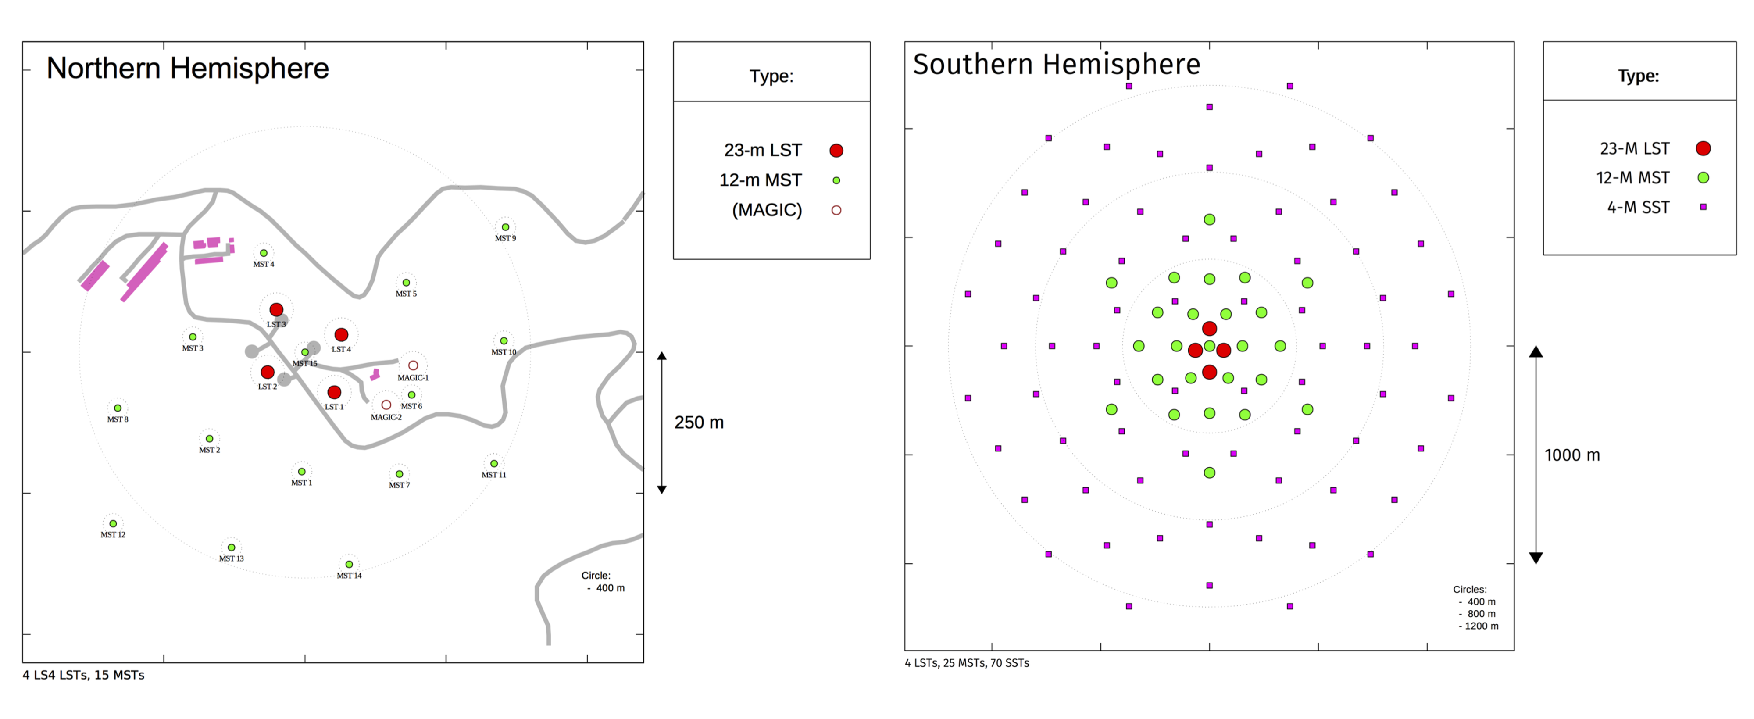
\includegraphics[width=1\textwidth]{Pictures/Array-Layouts.pdf}
  \caption{Array layout selected for \gls{cta} from \cite{CTAPerformance}. Left is Northern site where also \gls{magic} telescopes are located. Right is Southern location.}
    \label{fig:arraylayout}
\end{figure}

The baseline design for Southern observatory forsees 4 \glspl{lst}, \glspl{mst} and 70 \glspl{sst}. It will be dedicated to the study of galactic sources which emit the most energetic $\gamma$-rays to reach the Earth. Because of the extremely low fluxes, it will cover very a large area ($\sim4$ km$^2$), achieved thanks to the large number of \glspl{sst}, to capture as many events as possible.\\
The Northern observatory will mainly observe extragalctic sources and transient events from which only the less energetic photons reach the Earth due to absorption (see section \ref{sec:absorption}). The final configuration will consist on 4 \glspl{lst} and 15 \glspl{mst}.

The performance of \gls{cta} has been evaluated in terms of the best results for the observation of a point source located at the centre of the field of view of telescopes cameras. A set of metrics are taken into account: Effective collection area, residual cosmic-ray background rate, angular resolution and differential sensitivity. Usually they are calculated after applying cuts in \textit{gammaness} and $\theta^2$ optimized to maximize sensitivity for a set of typical observation times. Gammaness is referred to the gamma-hadron separation of shower events, events with higher gammaness are more likely to be produced by a $\gamma$-ray instead of a hadron. The angle $\theta^2$ is the square of the angle between the reconstructed source position and the true source position.
An overview of the mentioned metrics for performance evaluation is the following:\\

\begin{itemize}
\item \textbf{Effective collection area:} The effective collection area describes the area in which \gls{cta} is able to detect a shower from the point source. The effective collection areas for the assumed point sources are shown in figure \ref{fig:effarea}.\\

\begin{figure}[!htb]
\minipage{0.5\textwidth}
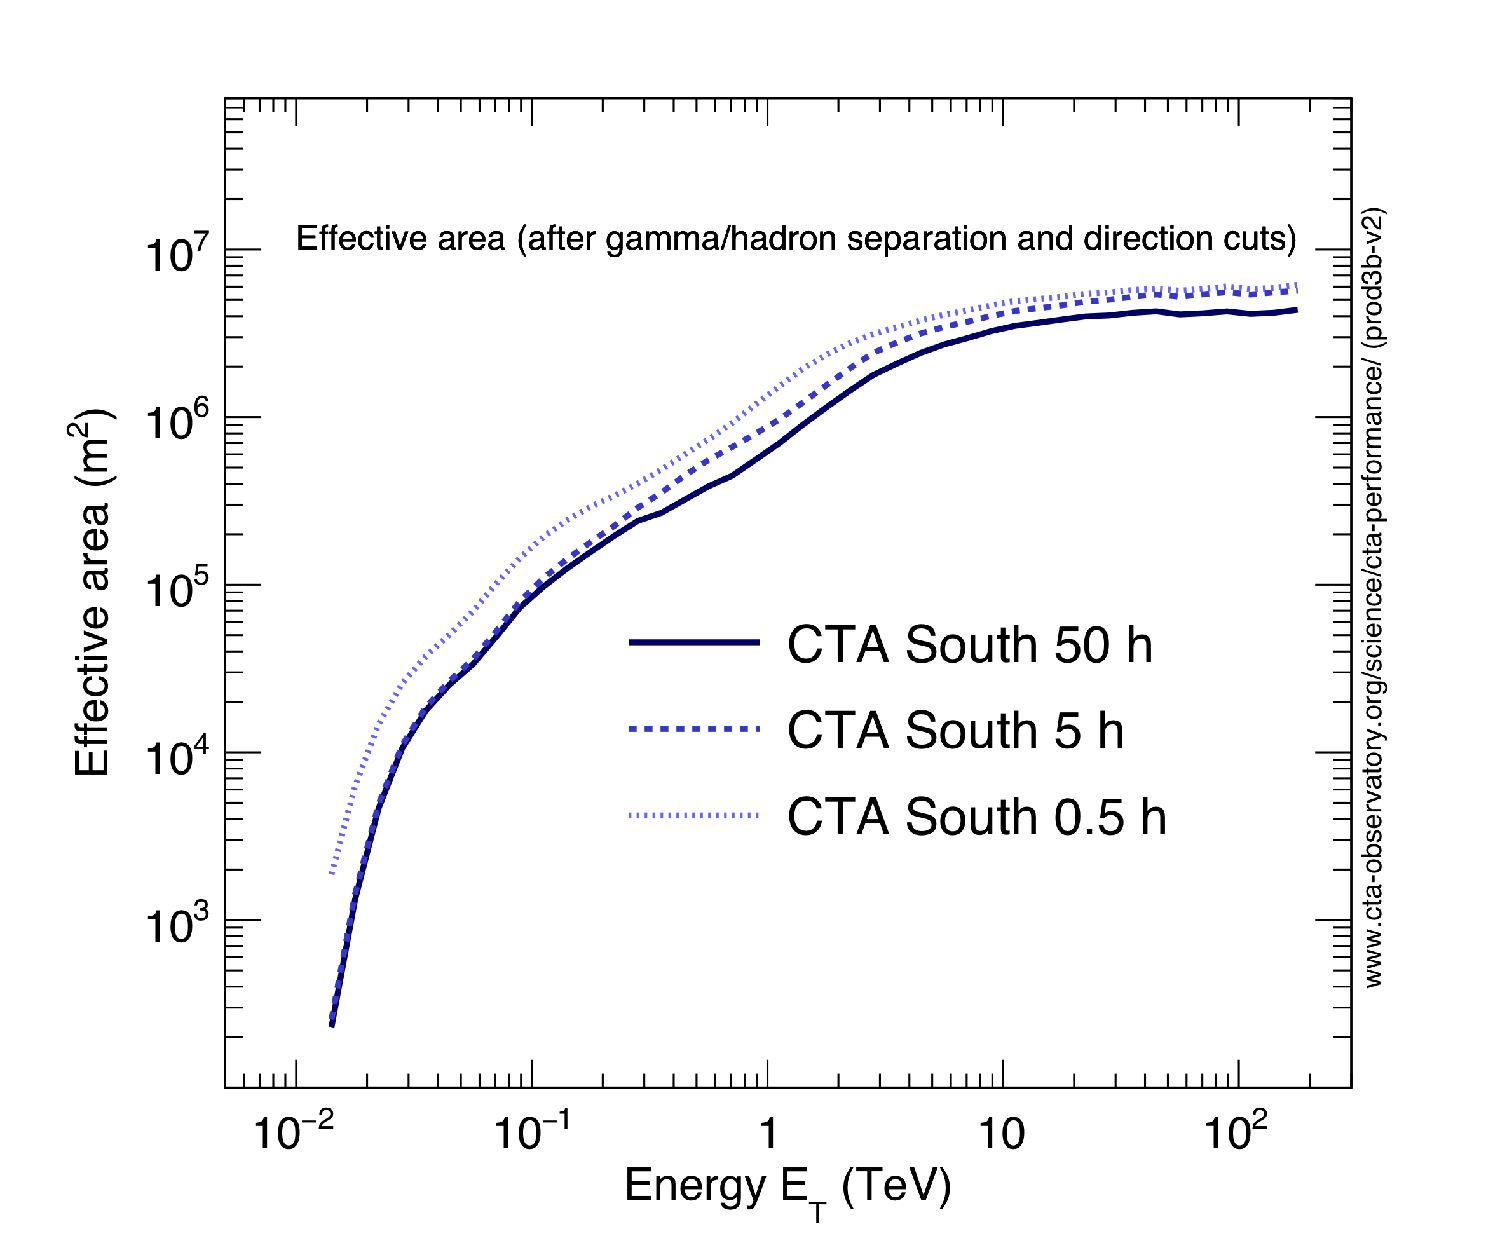
\includegraphics[width=\linewidth]{Pictures/CTA-Performance-prod3b-v2-South-20deg-EffectiveArea.pdf}
\endminipage\hfill
\minipage{0.5\textwidth}
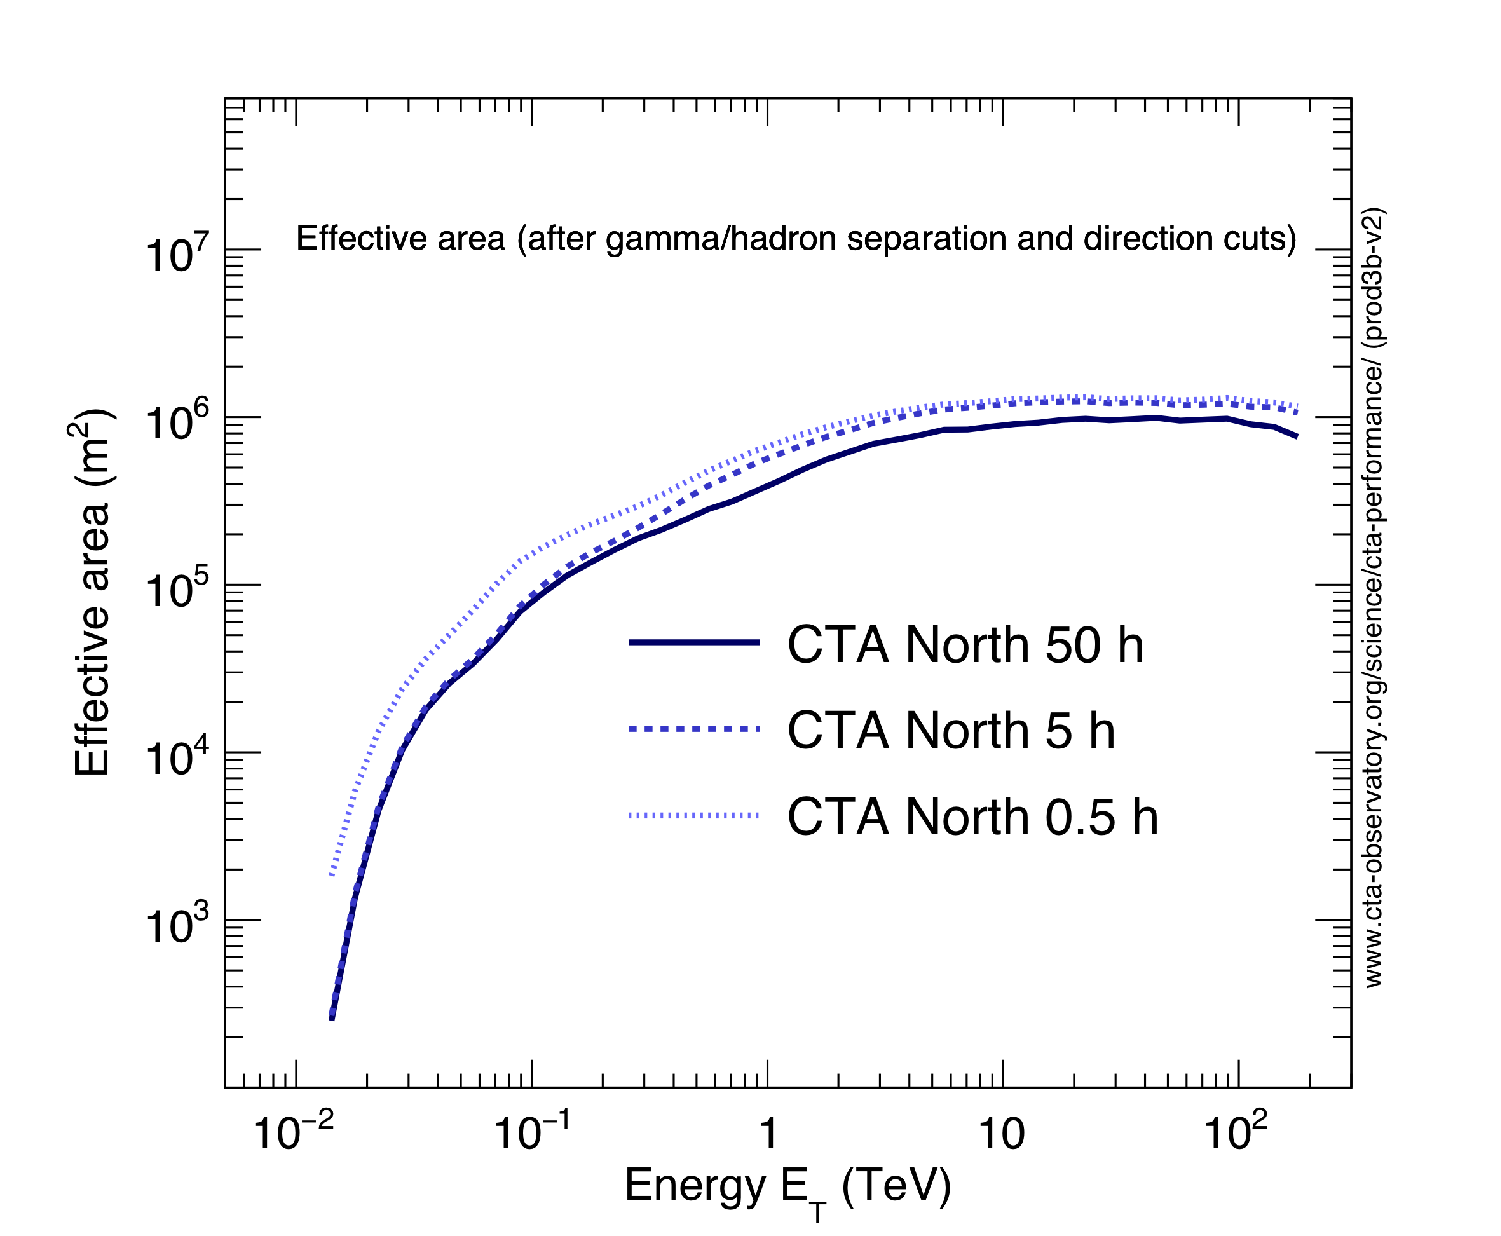
\includegraphics[width=\linewidth]{Pictures/CTA-Performance-prod3b-v2-North-20deg-EffectiveArea.pdf}
\endminipage\hfill
\caption{\label{fig:effarea}Effective collection area for point-like sources for CTA South(left) and CTA North (right) \cite{CTAPerformance}.}
\end{figure}

\item \textbf{Residual cosmic-ray background rate:} The ability of \gls{cta} to reject background events, meaning showers produced by \glspl{cr} instead of $\gamma$s is measured through the residual cosmic-ray background rate. The 99.9\% of the showers reaching the telescopes are produced by \glspl{cr}, so a good background rejection is a key requirement for \glspl{iact}. In figure \ref{fig:bkgrate} the (post-analysis) residual cosmic-ray background rate per square degree vs reconstructed $\gamma$-ray energy is shown. The rate is integrated in each bin, where five bins per decade has been taken. \gls{cta} have such strong background rejection capabilities that the majority of the background in the range 0.2-1.5 TeV is due cosmic-ray electrons and positrons \cite{2017ICRCCTAPerformance} which produce showers much more difficult to differentiate from electromagnetic showers than those produced by hadrons (see section \ref{sec:electroshowers}).\\

  \begin{figure}[!htb]
    \minipage{0.5\textwidth}
    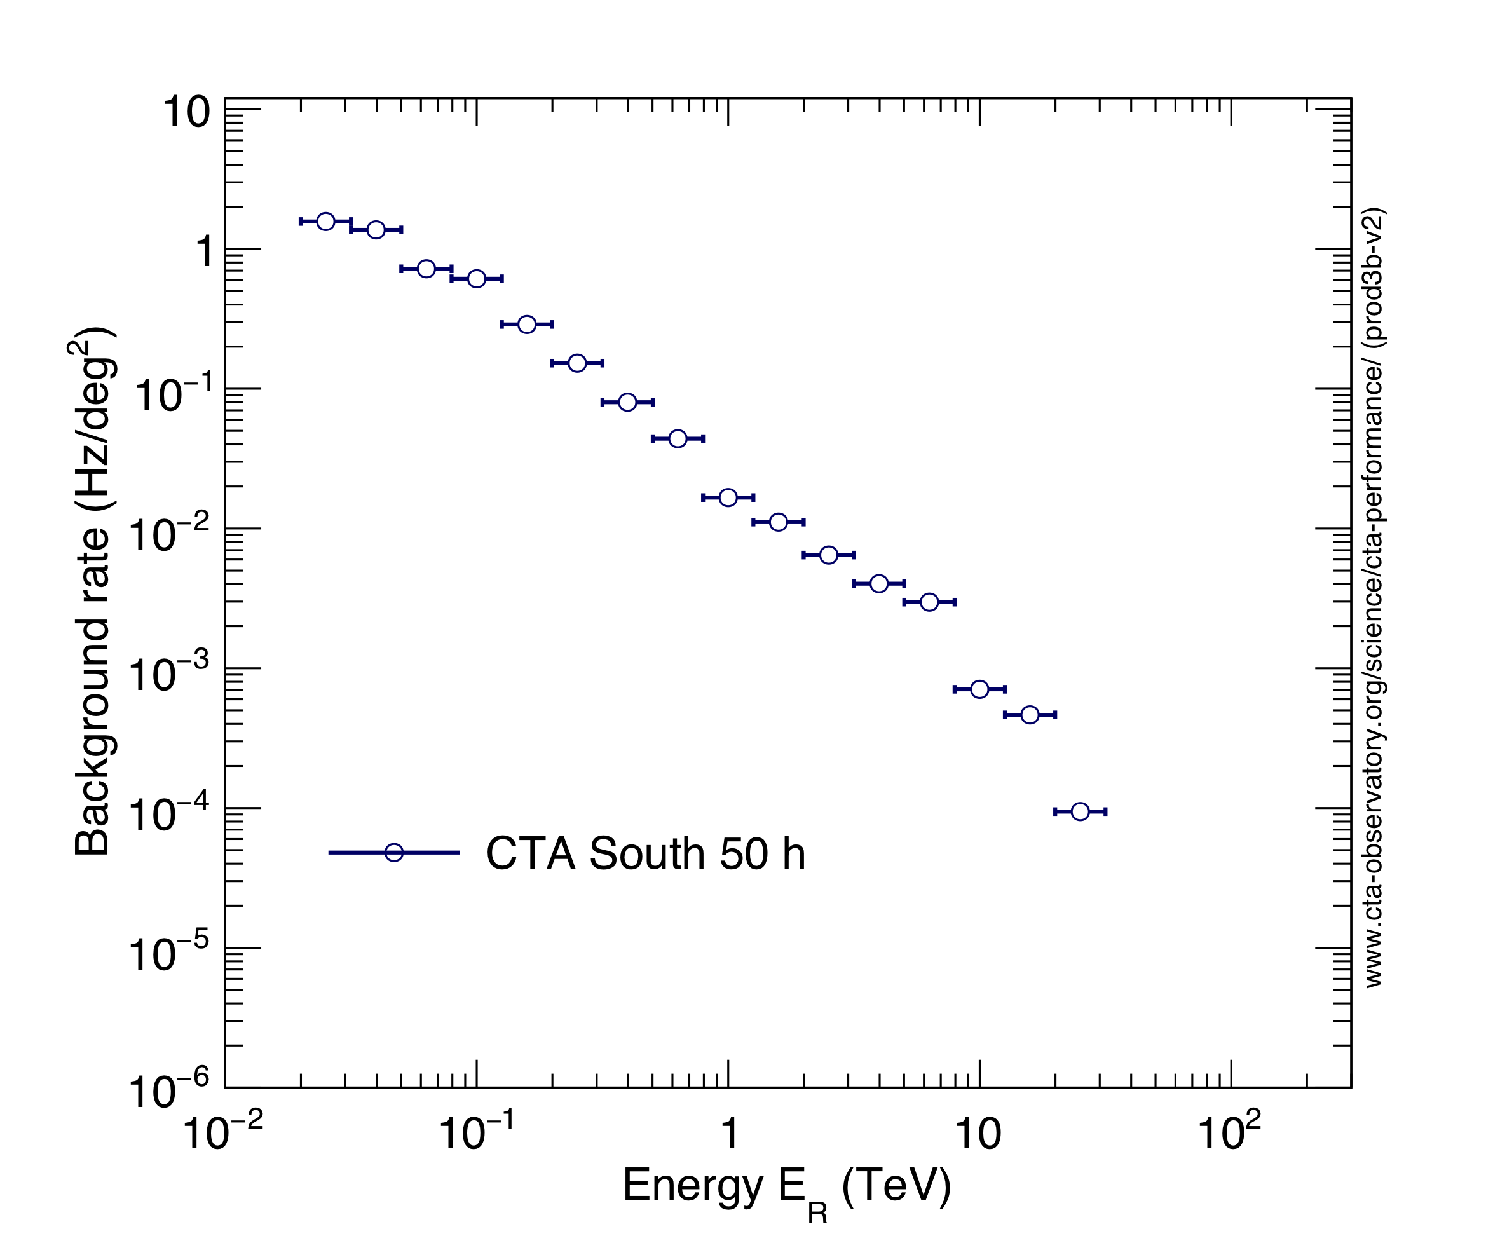
\includegraphics[width=\linewidth]{Pictures/CTA-Performance-prod3b-v2-South-20deg-BackgroundRateSquDeg.pdf}
    \endminipage\hfill
    \minipage{0.5\textwidth}
    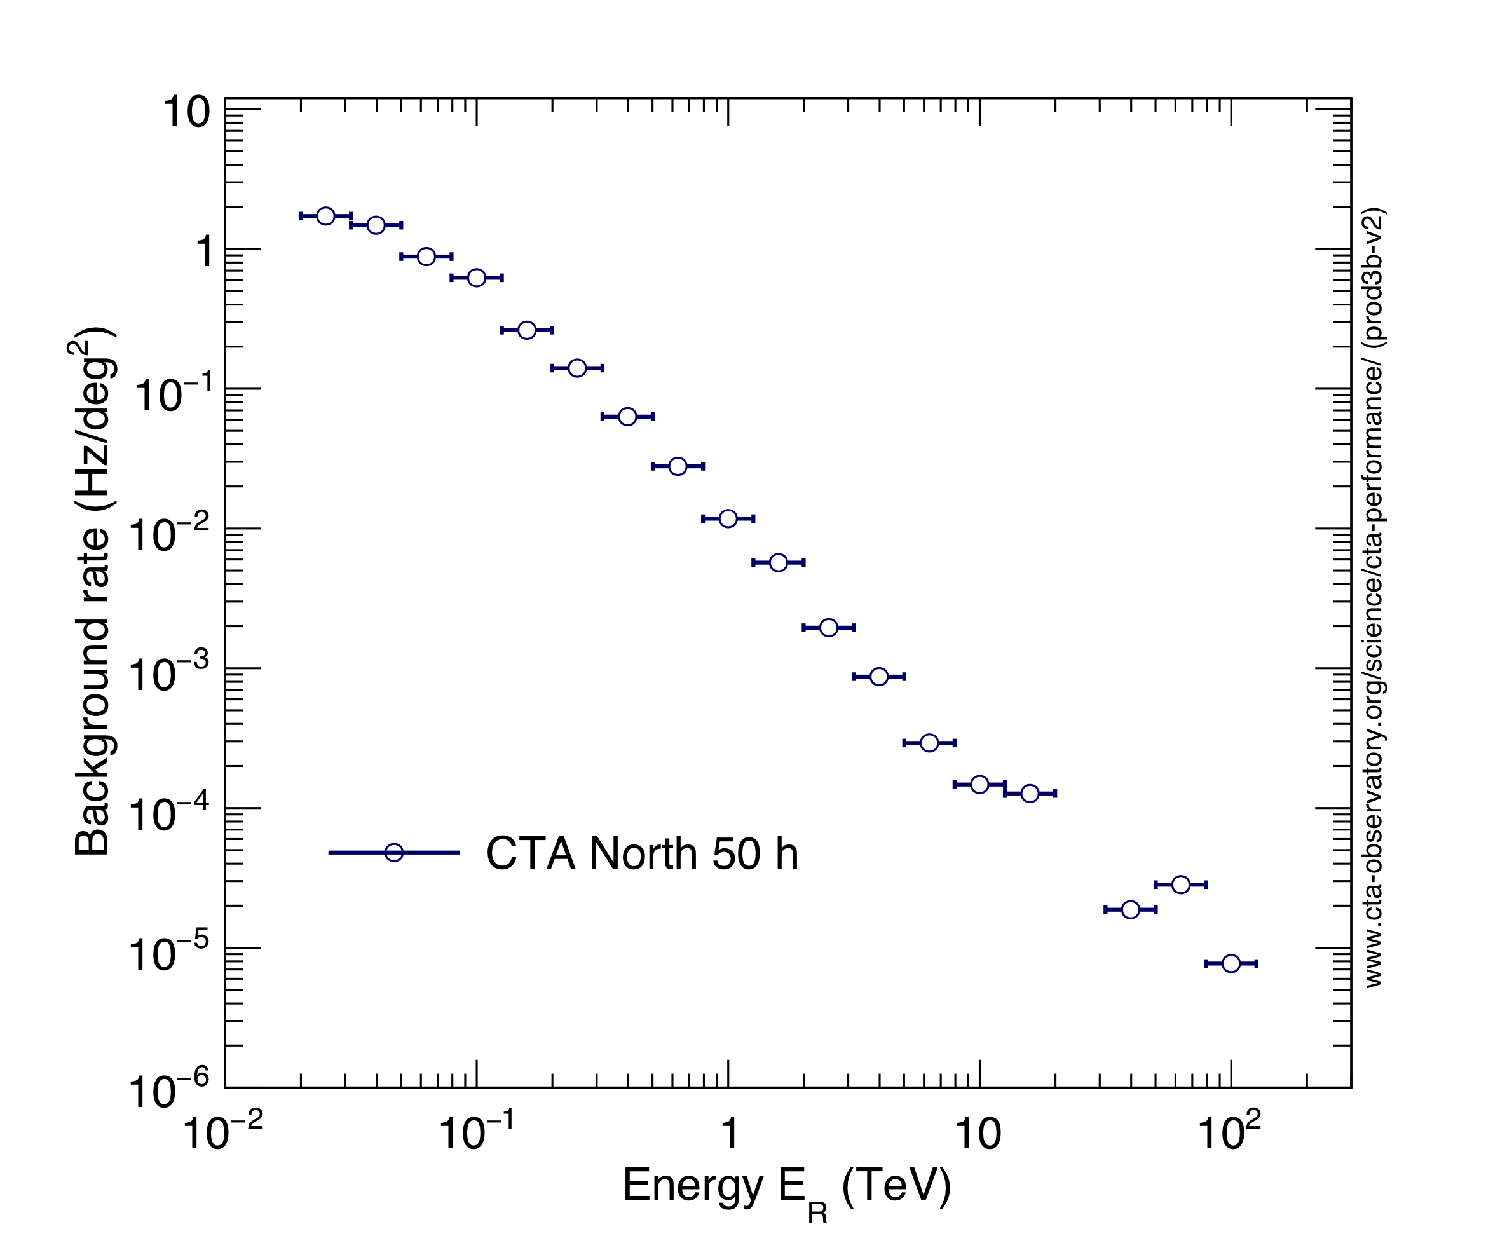
\includegraphics[width=\linewidth]{Pictures/CTA-Performance-prod3b-v2-North-20deg-BackgroundRateSquDeg.pdf}
    \endminipage\hfill
    \caption{\label{fig:bkgrate} Residual cosmic-ray background rate vs reconsctructed enregy for CTA South(left) and CTA North (right) \cite{CTAPerformance}.}
  \end{figure}
  
\item \textbf{Angular resolution:} The angular resolution is defined as the angle within which 68\% of reconstructed $\gamma$-rays fall, relative to their true direction. Figure \ref{fig:angres} show the angular resolution vs. reconstructed energy optimized for best point-source sensitivity. It is possible to improve angular resolution at expenses of collection area for a better study of morphological features of bright sources.\\
  
  \begin{figure}[!htb]
    \minipage{0.5\textwidth}
    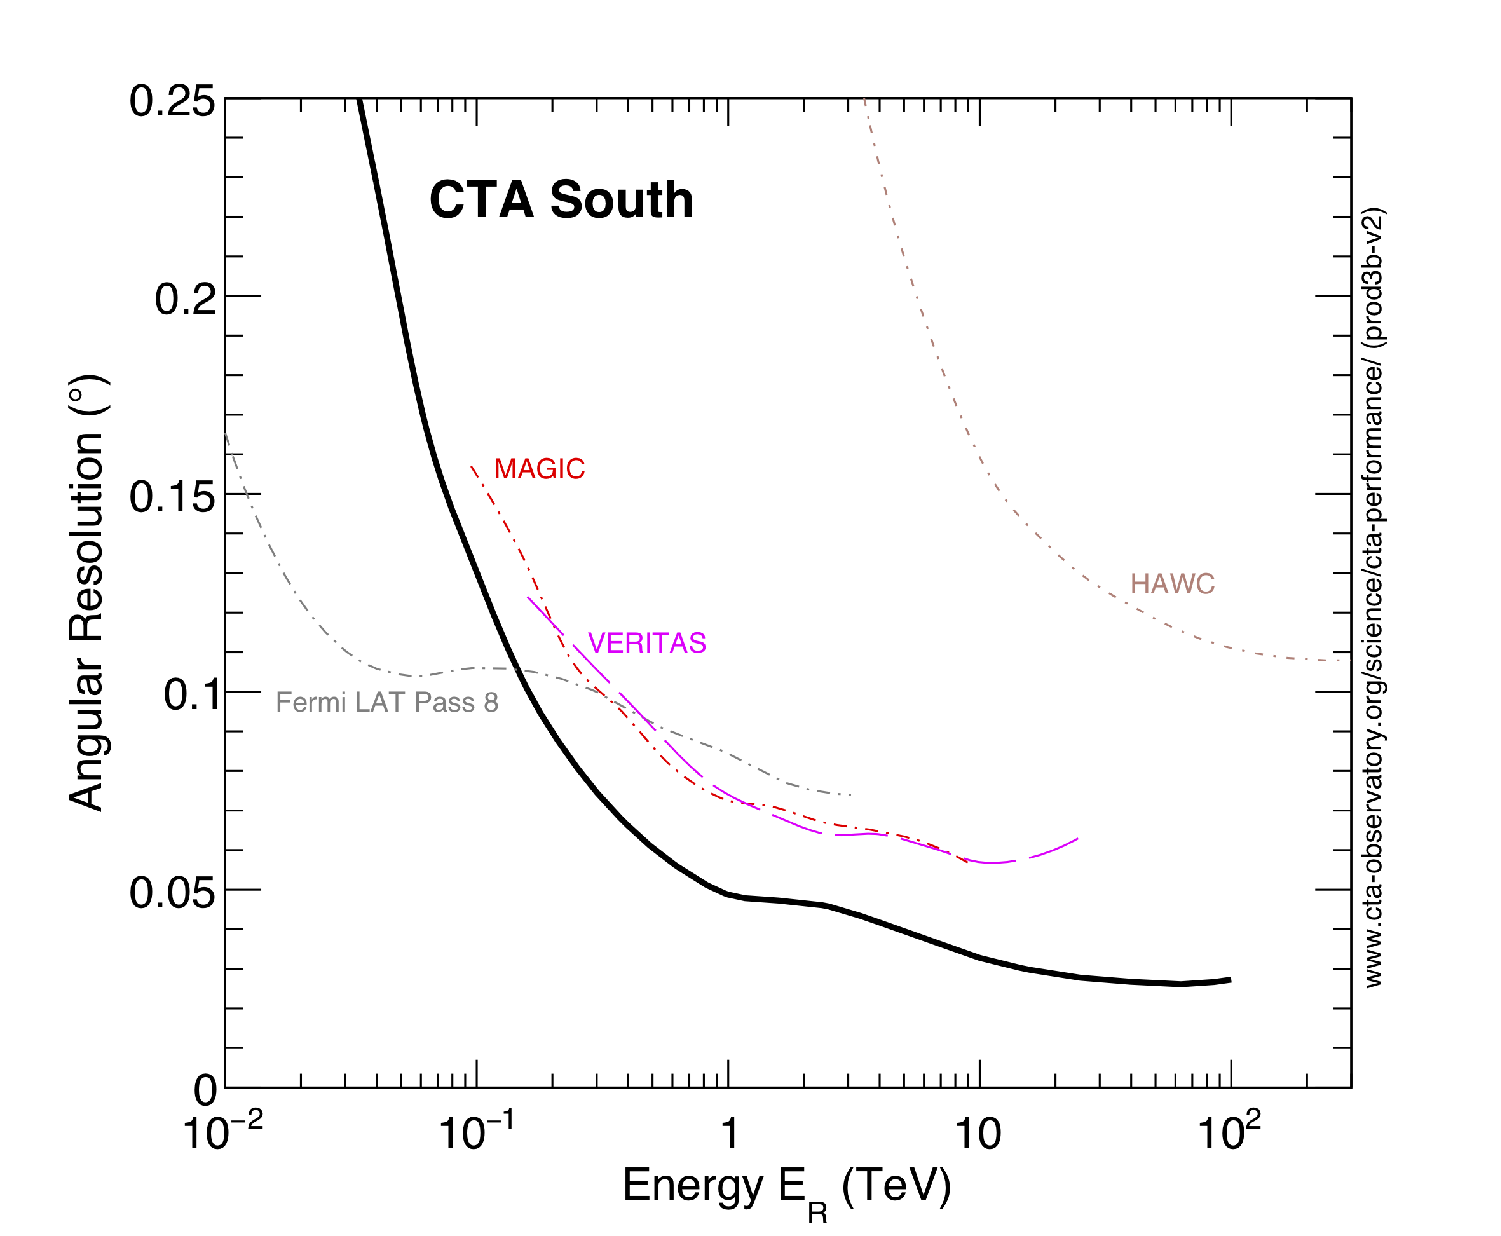
\includegraphics[width=\linewidth]{Pictures/CTA-Performance-prod3b-v2-Comparison-AngularResolution-OtherInstruments.pdf}
    \endminipage\hfill
    \minipage{0.5\textwidth}
    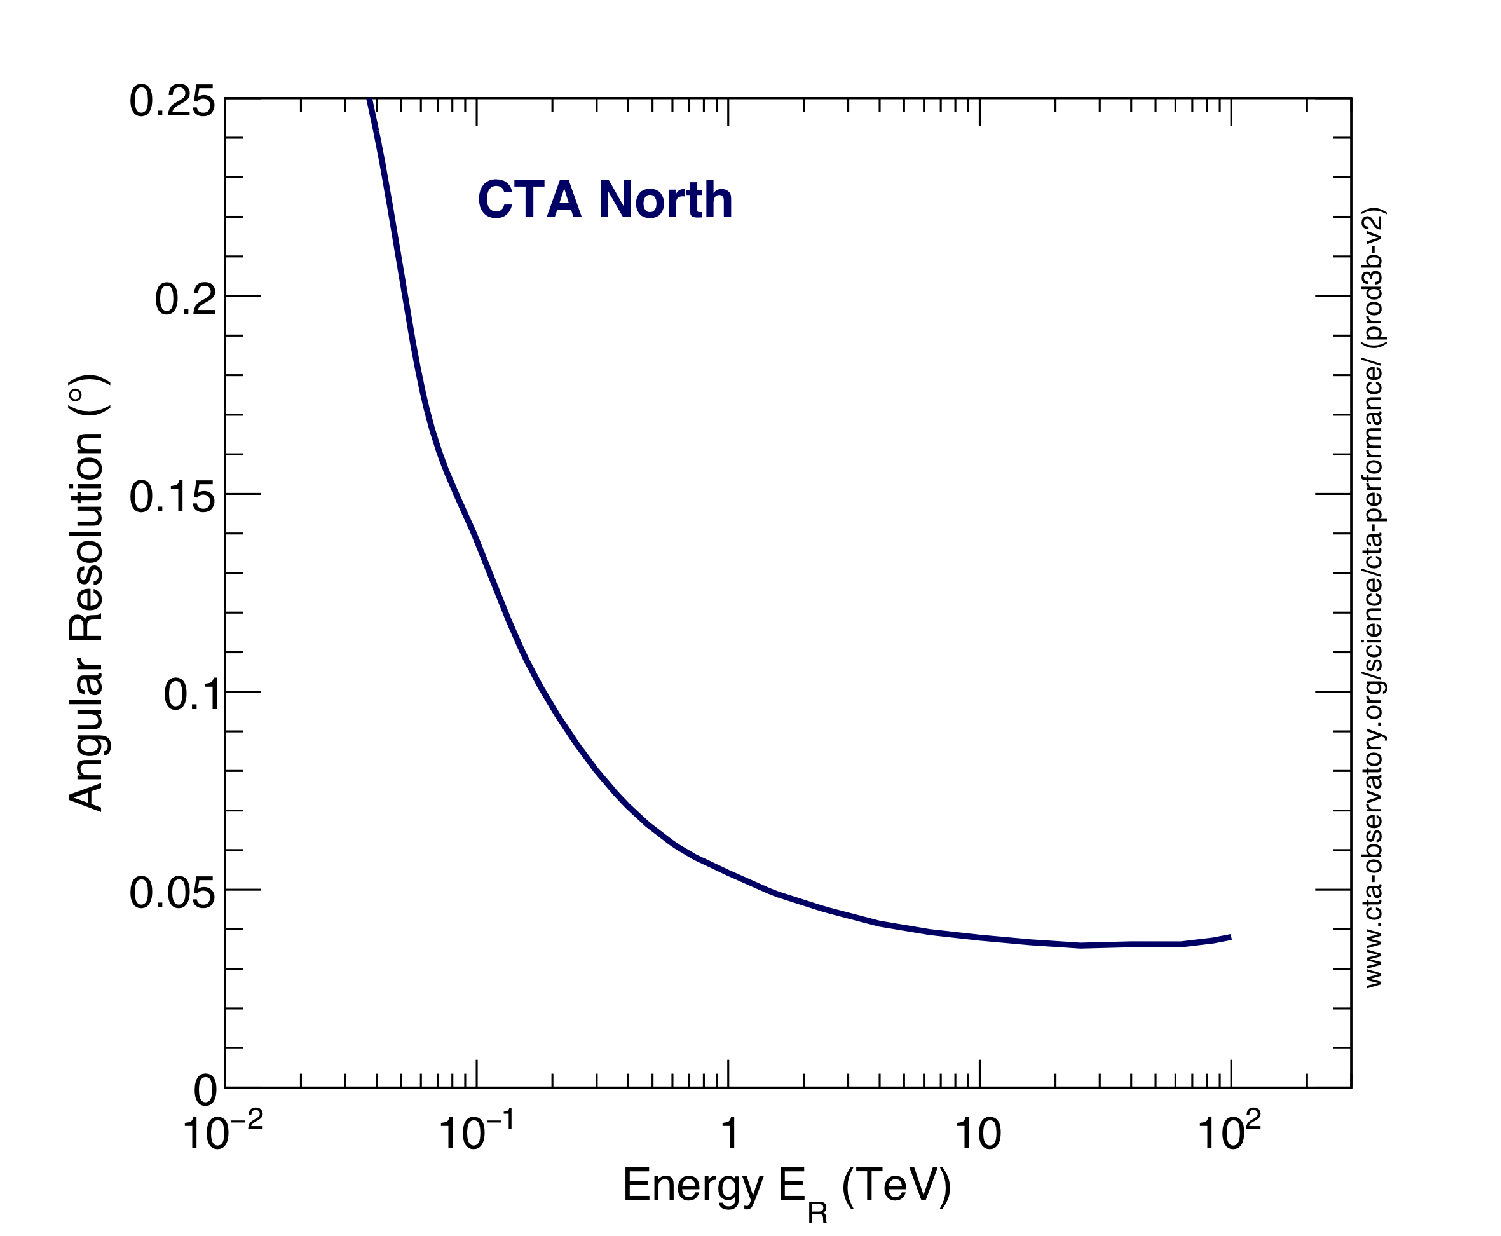
\includegraphics[width=\linewidth]{Pictures/CTA-Performance-prod3b-v2-North-20deg-AngularResolution.pdf}
    \endminipage\hfill
    \caption{\label{fig:angres} Angular resolution for CTA South compared to other experiments (left), and for CTA North (right) \cite{CTAPerformance}.}
  \end{figure}

\item \textbf{Energy resolution:} The energy resolution $\Delta E/E$ is obtained from the distribution $E_{rec}-E_{true}/E_{true}$, where $E_{true}$ and $E_{rec}$ are the true and reconstructed energies of $\gamma$-ray events. It is defined as the half-width of the interval around 0 which contains the 68\% of the distribution. The energy resolution of \gls{cta} as a function of reconstructed energy is shown in figure \ref{fig:energyres}. Note that for the range of 1-10 TeV the energy resolution is well below the required 10\%.\\
    
  \begin{figure}[!htb]
    \minipage{0.5\textwidth}
    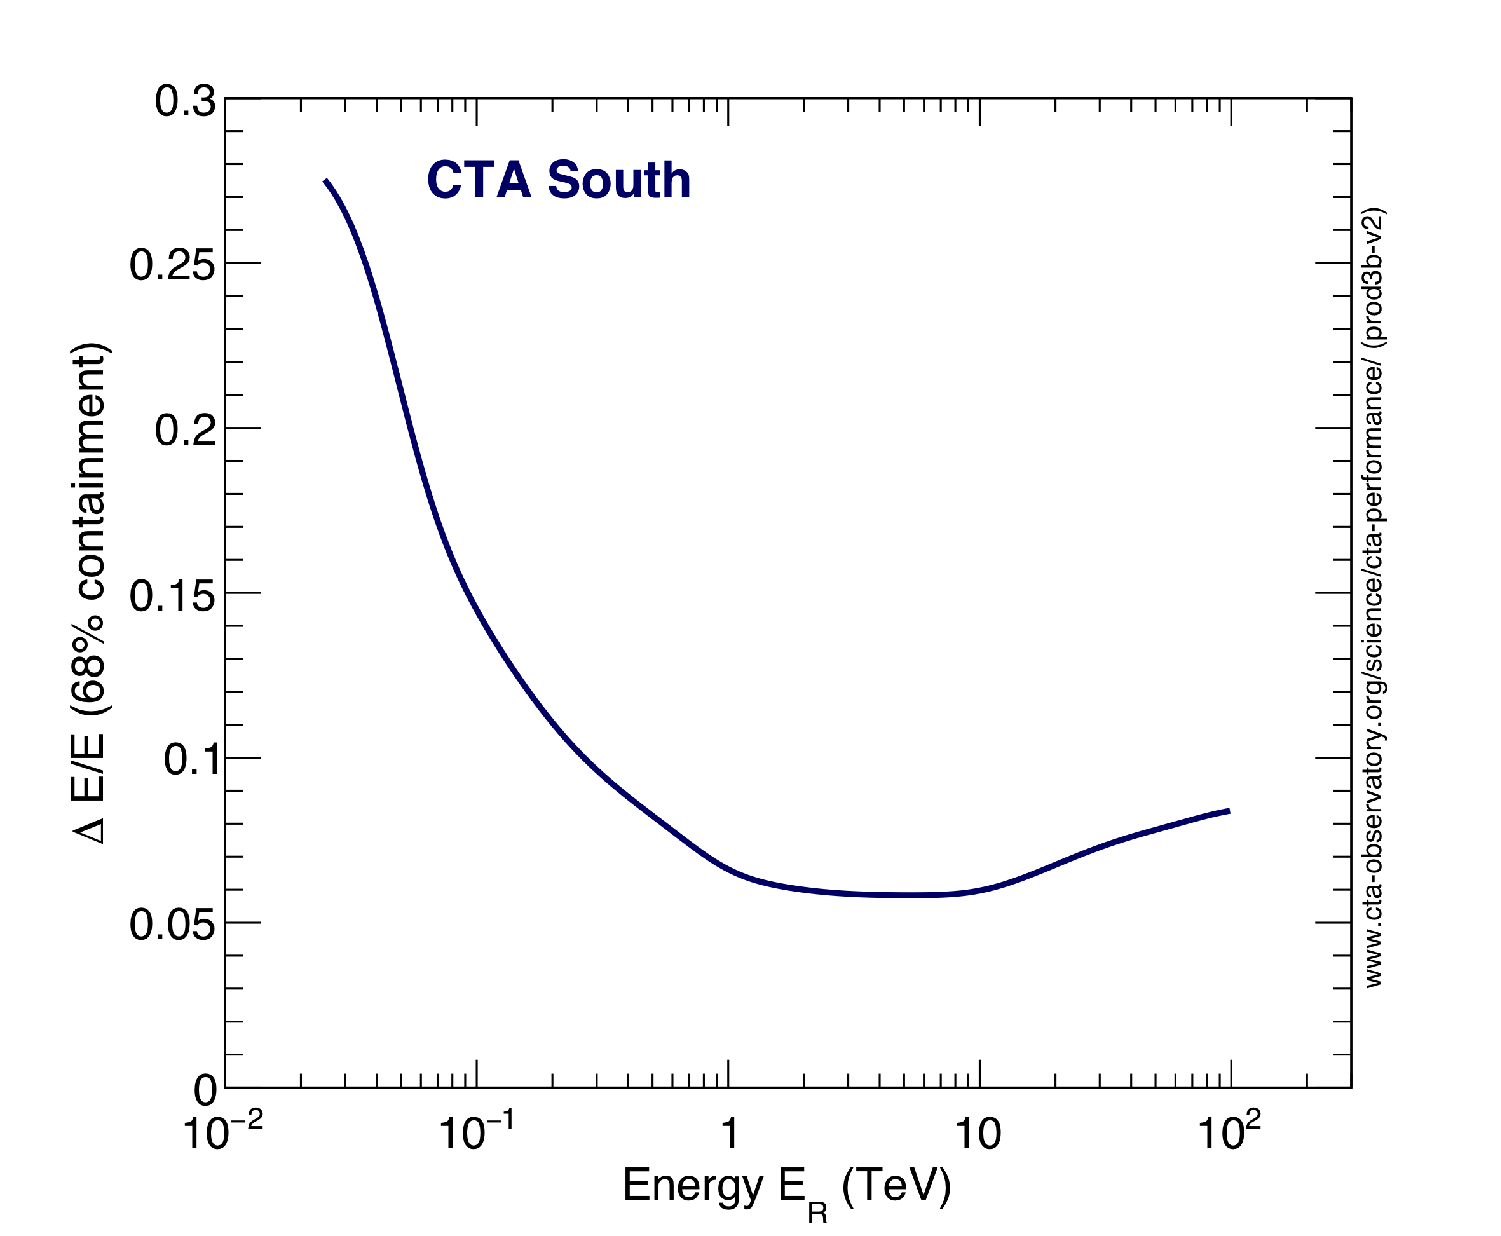
\includegraphics[width=\linewidth]{Pictures/CTA-Performance-prod3b-v2-South-20deg-EnergyResolution.pdf}
    \endminipage\hfill
    \minipage{0.5\textwidth}
    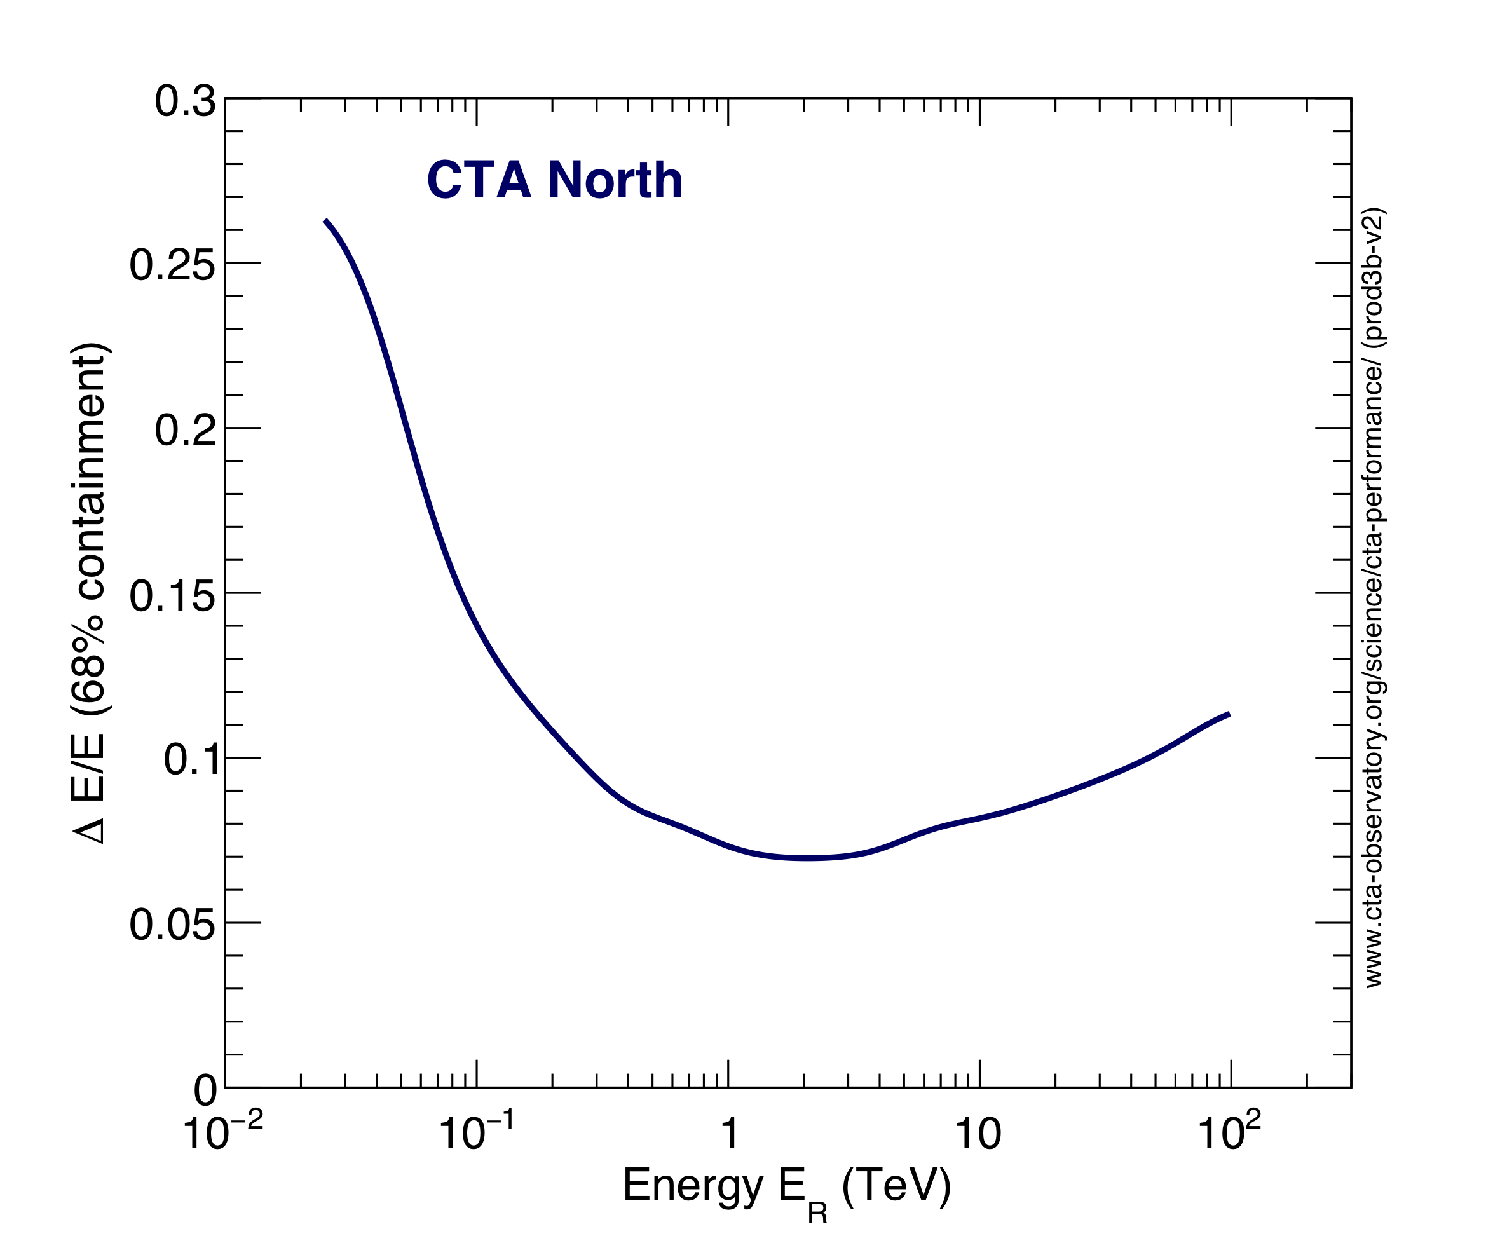
\includegraphics[width=\linewidth]{Pictures/CTA-Performance-prod3b-v2-North-20deg-EnergyResolution.pdf}
    \endminipage\hfill
    \caption{\label{fig:energyres} Energy resolution vs reconstructed energy for CTA South (left) and CTA North (right) \cite{CTAPerformance}.}
  \end{figure}
  
\item \textbf{Differential sensitivity:} The most important feature at evaluating the performance is the differential sensitivity, which indicates the minimum flux needed by \gls{cta} to detect a point-like source at $5\sigma$. The sensitivity is calculated in five energy bins per decade, where it is required that at least 10 $\gamma$-rays are detected and the signal to background ratio is al least 1/20. The cuts in gammaness and source direction ($\theta^2$) are optimized to improve this quantity. The differential sensitivity of \gls{cta} compared to that of other instruments for 50h observation time was shown in figure \ref{fig:ctaperformance}.\\
  
\end{itemize}

\section{CTA Telescopes} \label{sec:ctatelescopes}

While all telescopes share a basic design concept, each of them have particlar features to accomplish the performance requirements for \gls{cta}. In general, subsystems of \glspl{iact} are divided in \textbf{structure}, \textbf{optics} (mirros) and \textbf{camera}. 
In this section an overview of these subsystems and the particularities of each of the three types of \gls{cta} telescopes is given. 

\subsection{Large Size Telescope (LST)}

The purpose of the \gls{lst} is to enhance the sensitivity of \gls{cta} at low energies, reaching an effective threshold down to 20-30 GeV. This energy range has a particular interest because it covers the barely explored gap between the highest energies detcted by satellite experiments, and the lowest by \glspl{iact}. The main science goals for \glspl{lst} is to observe high redshift \glspl{agn}, \glspl{grb}, pulsars and galactic transients. The first prototype for the \glspl{lst} (\gls{lst}1) has been installed in the CTA North site, in La Palma island and is currently being commissioned.\\
A detailed description of \gls{lst} subsystems can be found in \cite{2013LST}, next sections offer a summary of the most remarckable features of the telescope.\\

\subsubsection{\gls{lst} Structure}

The structure of the telescope is divided in several parts: The azimuth system and substructure, the mirror support dish, the elevation system and, camera support structure and the drive system. All parts of the structure are specially designed to make the telescope lightweight and ensure fast repositioning in the case of an alert of a transient event (mainly \glspl{grb}).\\
The azimuth system allows the telescope to turn around its vertital axis. It consist in a circular rail of 24m diameter where six boogies support the structure of the telescope. The azimuth structure of the telescope is a space framed structure made of \gls{cfrp} tubes. Its design is very similar to that of \gls{magic} telescopes, but much lighter. The mirror support dish is a double layer space frame made of \gls{cfrp} tubes arranged in a tetrahedral structure. The diameter of the dish is 23 m and the focal length is 28 m. The elevation system consist on a structure made of heavier steel tubes, located in the backside of the dish, to help compensate the weight of the telescope structure. The camera support structure consists on an arch with three curve sections on each arm, made of \gls{cfrp}. A total of 26 ropes shiften the structure. The arch holds the camera frame, where the camera and the square lids are fixed. The drive system, designed to ensure a fast and precise repositioning, consist on 4 synchronous motors capable to supply a total mechanical power of 190 Kw to move the structure in azimuthal axis and elevation. The different parts of the structure are shown in figure \ref{fig:LST}.
    
  \begin{figure}[!htb]
    \minipage{0.5\textwidth}
    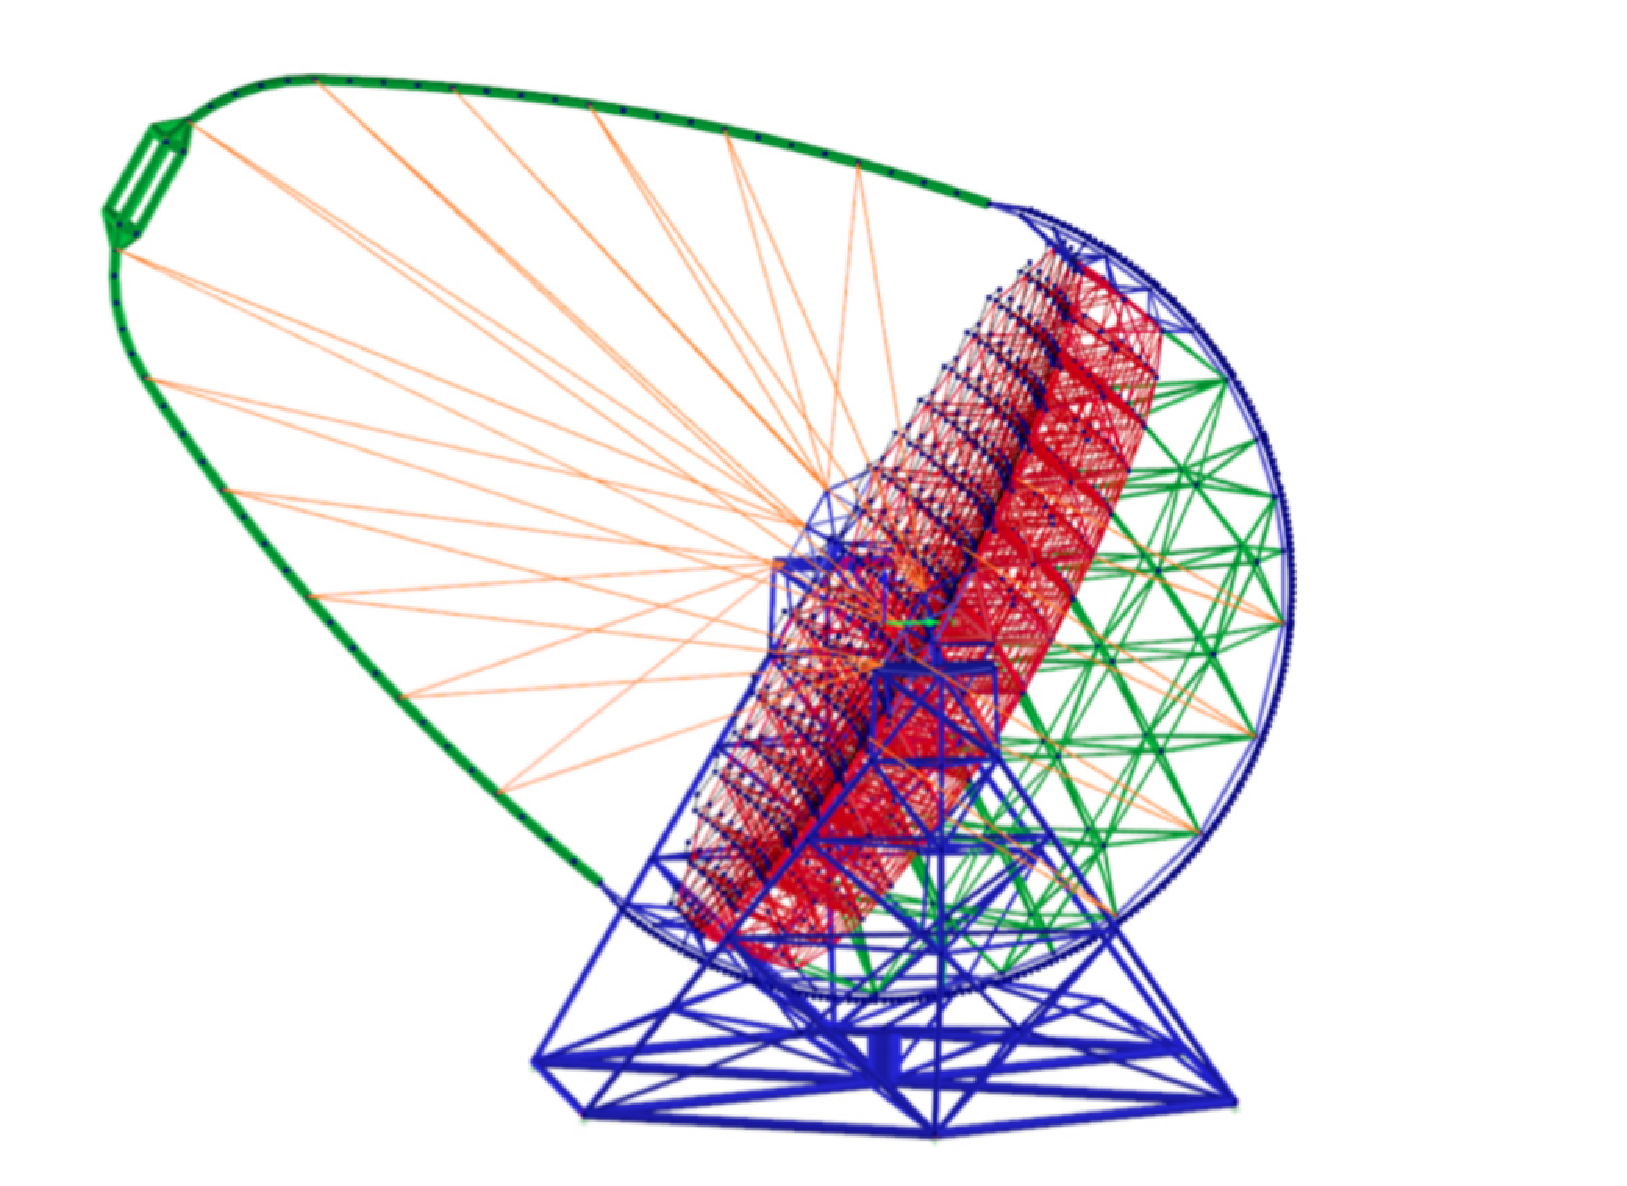
\includegraphics[width=\linewidth]{Pictures/LSTstructure.pdf}
    \endminipage\hfill
    \minipage{0.5\textwidth}
    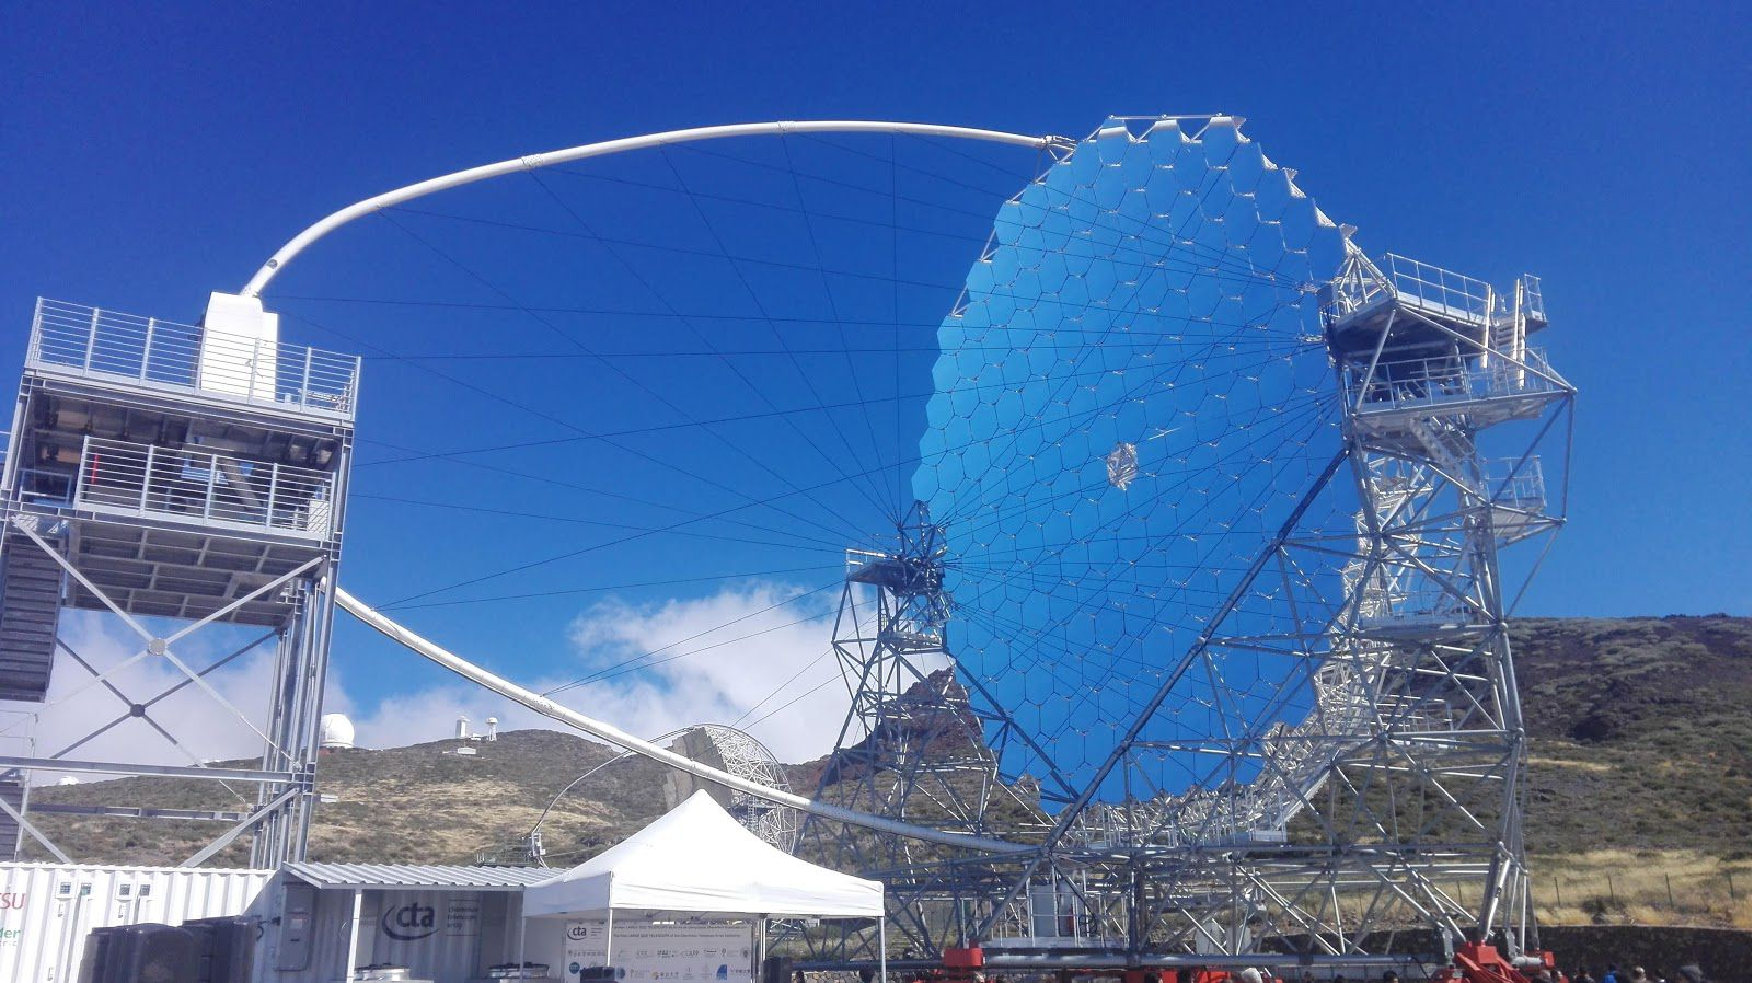
\includegraphics[width=\linewidth]{Pictures/LST1.pdf}
    \endminipage\hfill
    \caption{\label{fig:LST} Left: Simplified diagram of the structures of \gls{lst} without bogies, mirrors and camera. Azimuth substructure is blue color, the elevation system and the camera support structure are shown in green color and the mirror dish is red color, from \cite{2013LST}. Right: Photo of the first LST installed in CTA North site (Roque de los Muchachos Observatory, La Palma, Spain).}
  \end{figure}
  
  \subsubsection{\gls{lst} Optics}

  The mirror structure is a parabolic shape of 28 m diameter, composed of 198 hexagona mirrors of spherical shape. The structure is made in a way that it guarantees the isochronousity of the optics. The mirrors are manufactured using the cold slump technique where a sandwich structure is composed a soda-lime glass sheet, an aluminum honeycomb box and another glass sheet\cite{2017LST}.
Mirrors are fixed to the telescope structure by three knots, two of them mounted on actuators which allow to adjust each mirro panel in two directions. The \textit{active mirror control} system controls these actuaros in order to vary focal distance and focusing, to account for the possible deformations and bending of the telescope structure. Each mirror segment account for an ifnrarred laser, and two more lasers are mounted in the center of the disk, which constantly point to the left and right of the camera. The directional offset of the mirror facets can be estimated by taking pictures of the spots on a target in fornt of the camera with a high resolution IR CCD camera located in the center of the dish. The achievable positioning resolution can reach $< 5 \mu m$ \cite{2013LST}.
  
  \subsubsection{\gls{lst} Camera}

  The camera focal plane instrumentation consist on 256 modules each of one with seven \glspl{pmt}, making a total of 1855 pixels. The \glspl{pmt} are mounted with a 50mm spacing, so in order to collect all the light arriving to the camera, they are surrounded by hexagonal light guides made of a very reflective material (3M ESR). The \gls{pmt} model is Hamamatsu R11920-100-20, specially developed to reach high quantum efficiency (42\%) and low after pulse rates, which go below 0.02 \% above 4 photoelectrons. Each module with seven photodetectors has one readout system based on the \gls{dsr4}. The signal sampled at $\mathcal{O}$(GHz) is divided in three channels: high gain and low gain channels which are connected to the \gls{dsr4} chips and the trigger channel \cite{2017LST}. The two level trigger electronics (L0 and L1) are mounted on a mezzanine. A slow control board montors the \glspl{pmt} and analogue backplanes are dedicated to trigger and clock propagation.  
  The mechanical structure of the camera consist on several parts shown in figure \ref{fig:LSTcammech}. The modules of seven \gls{pmt} are coupled in ensembles named clusters, which are inserted in the load bearing structure. Slits in the back of the load bearing structure allow to connect the cluster readout electronics to the  backplanes. The design of such modular structures guarantee an easy access to individual modules in case any repair is necessary, allowing to disconect and extract one module while the rest of the camera is functioning.
  The load bearing structure is mounted inside a tubular structure which holds the camera external walls, doors and interfaces with the camera frame. In the front part of the camera there is the front window which can be totally covered by a shutter to avoid the entrance of sunlight during the day which could damage \glspl{pmt}. In the back part of the camera lies all the cabling and auxiliary electronics. The total dimensions of the camera is $2.9\times2.9\times 1$m$^3$ and the weight is less than 2000 kg. Since all the electronics are stored inside the camera, all the structure was designed to accomplish a series of requirements related to the exposure to environental conditions such as the protection to the entrance of dust, water and sunlight and guarantee a stable temperature between 20ºC to 40ºC \cite{2013LSTCamMech}. Temperature regulation is possible thanks to a \textit{cooling system} consisting on a water cooling system based on cold plates and a temperature controlled air flow cooling system.\\
 An \textit{access tower} allow the access to the camera during day time operations when the telescope rests in park position, and also acts as an anchor in case of strong winds. 

\begin{figure}
\centering
 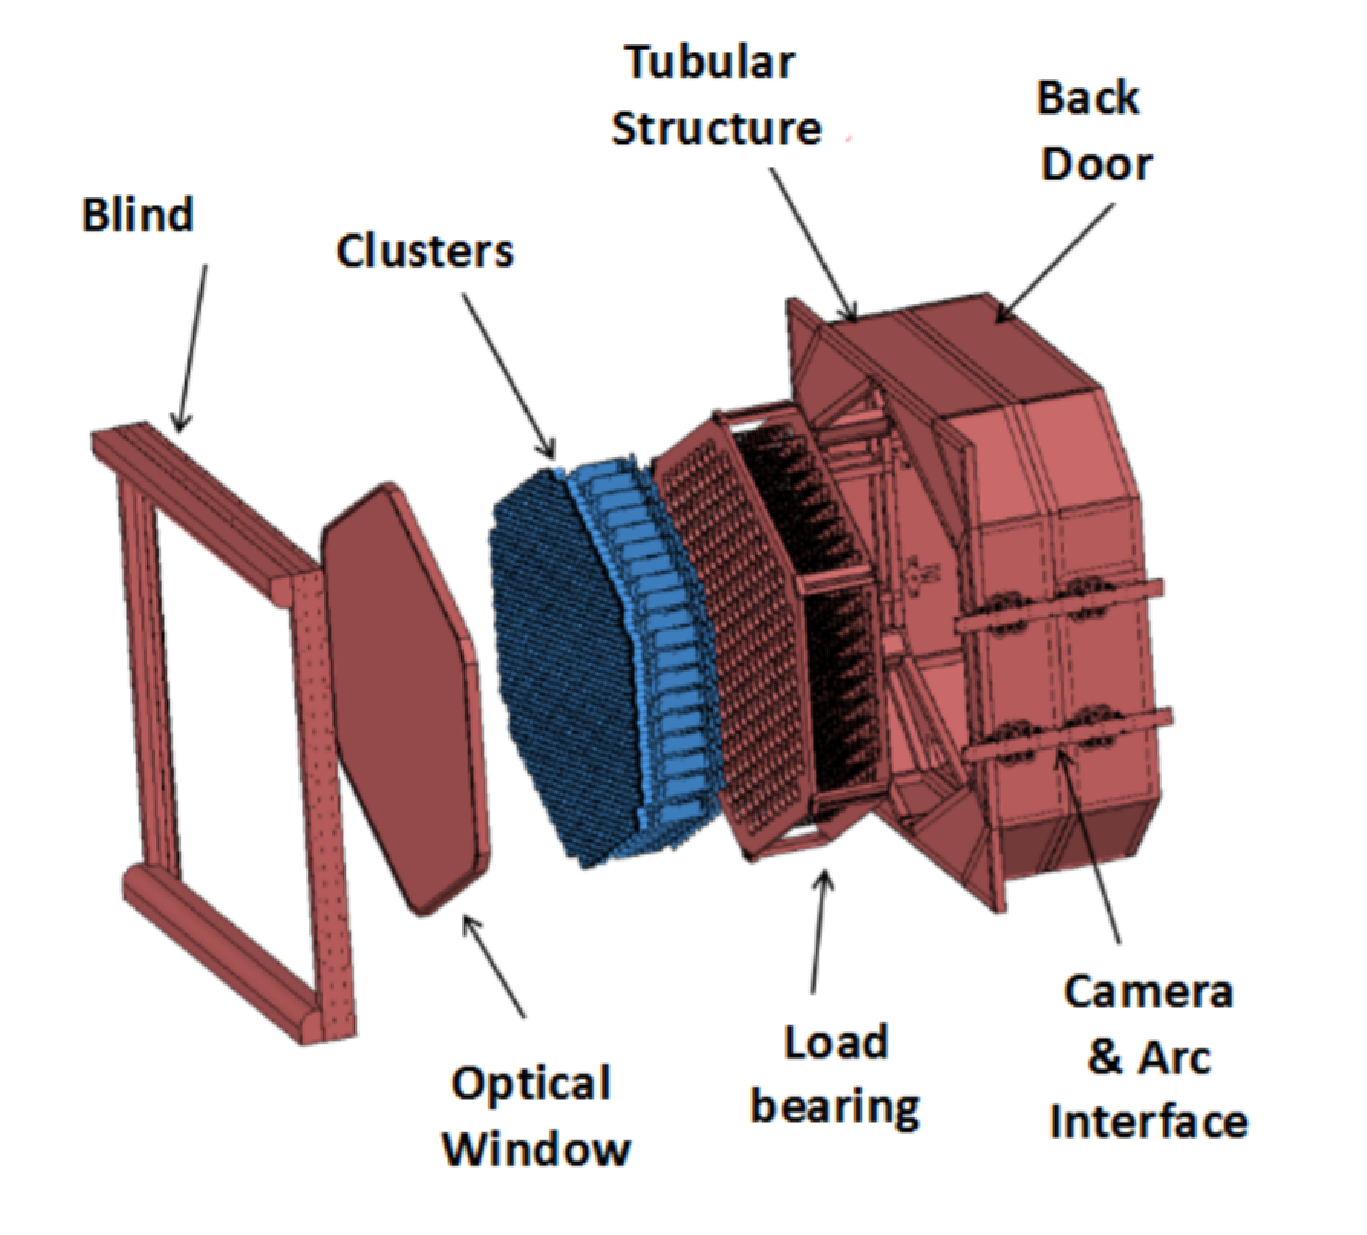
\includegraphics[width=0.7\textwidth]{Pictures/LSTcamerastructure.pdf}
  \caption{Different camera mechanical elements from \cite{2013LSTCamMech}.}
    \label{fig:LSTcammech}
\end{figure}

\subsection{Medium Size Telescope (MST)} \label{sec:MST}

\glspl{mst} will cover the core energy range of \gls{cta} observatory, from 100 GeV to $\sim 10$TeV. This is the range generally covered  by current \glspl{iact} so the improvements in sensitivity will come from the large area covered and the better image reconstruction due to the larger number of telescopes (15 in the north, 25 in the south).
Currently two approaches to the \gls{mst} design are carried on. The first is a 12 m diamater diameter modified Davis-Cotton optical layout very similar to that of \gls{veritas} and \gls{hess}. The first prototype of this type, the \gls{dcmst} \cite{2017SCMSTstatus}, has been built in Adlershof, Germany, ans is currently in commisioning phase. There are also two different camera designs for \gls{dcmst}: \textit{FlashCam} and \textit{NectarCAM}, which characteristics will be discussed in this section.
The second design uses a novel technique never built before \gls{cta}, with a 10 m diameter Schwarzschild–Couder \cite{2017SCMSTstatus} optics accounting of two mirrors, and a novel \gls{sipm} camera. The prototype for this telescope has been built in the Fred Lawrence Whipple Observatory, in Arizona. 
A detailed report of the status of the \glspl{mst} as of July 2019 can be found \cite{2019MSTreport}. A summary on the different parts of the telescopes is given in this section.

\subsubsection{\gls{mst} Structure}

The structure of both telescope designs is similar with specific modifications for the optical system of the \gls{scmst} \cite{2017SCMSTstatus} as can be seen in figure \ref{fig:2MST}.
The main mechanical structure of the telescope is a cylindrical tower of 1.8 m diameter and 20 mm wall thickness. The tower is connected on top to the head of the telescope, that contains the azimuth bearing which allows the telescope to rotate in the horizontal axis, and the drive assemblies. It is possible yo access to the tower through a door at the base and in the inside, all electrical cabinets are stored distributed over three floors. A combination of ventilation and air conditioning system is used to keep the temperature within operation range.
The drive assemblies are designed to reach any object above 30º in elevation in less than 90s. It is divided in the azimuth drive subassembly and two elevation drive subassemblies, mounted in the left and right of the telescope.
To account for the possible sources of excitation, like wind gusts or structure flexibility, which can lead to oscillations of the structue an active vibration damping control is used to reduce their effect on the pointing accuracy of the telescope.
The dish structure is designed to host the mirrors and attached to it is the camera support structure \cite{2015DCMSTstatus}.
For the \gls{scmst}, the positioner is the same, but the optical support is very different to sustain the segmented aspheric primary and secondary mirrors, and the camera support structure, located in the focus of the secondary \cite{2018MSTandLSTstatus}.


\begin{figure}
\centering
 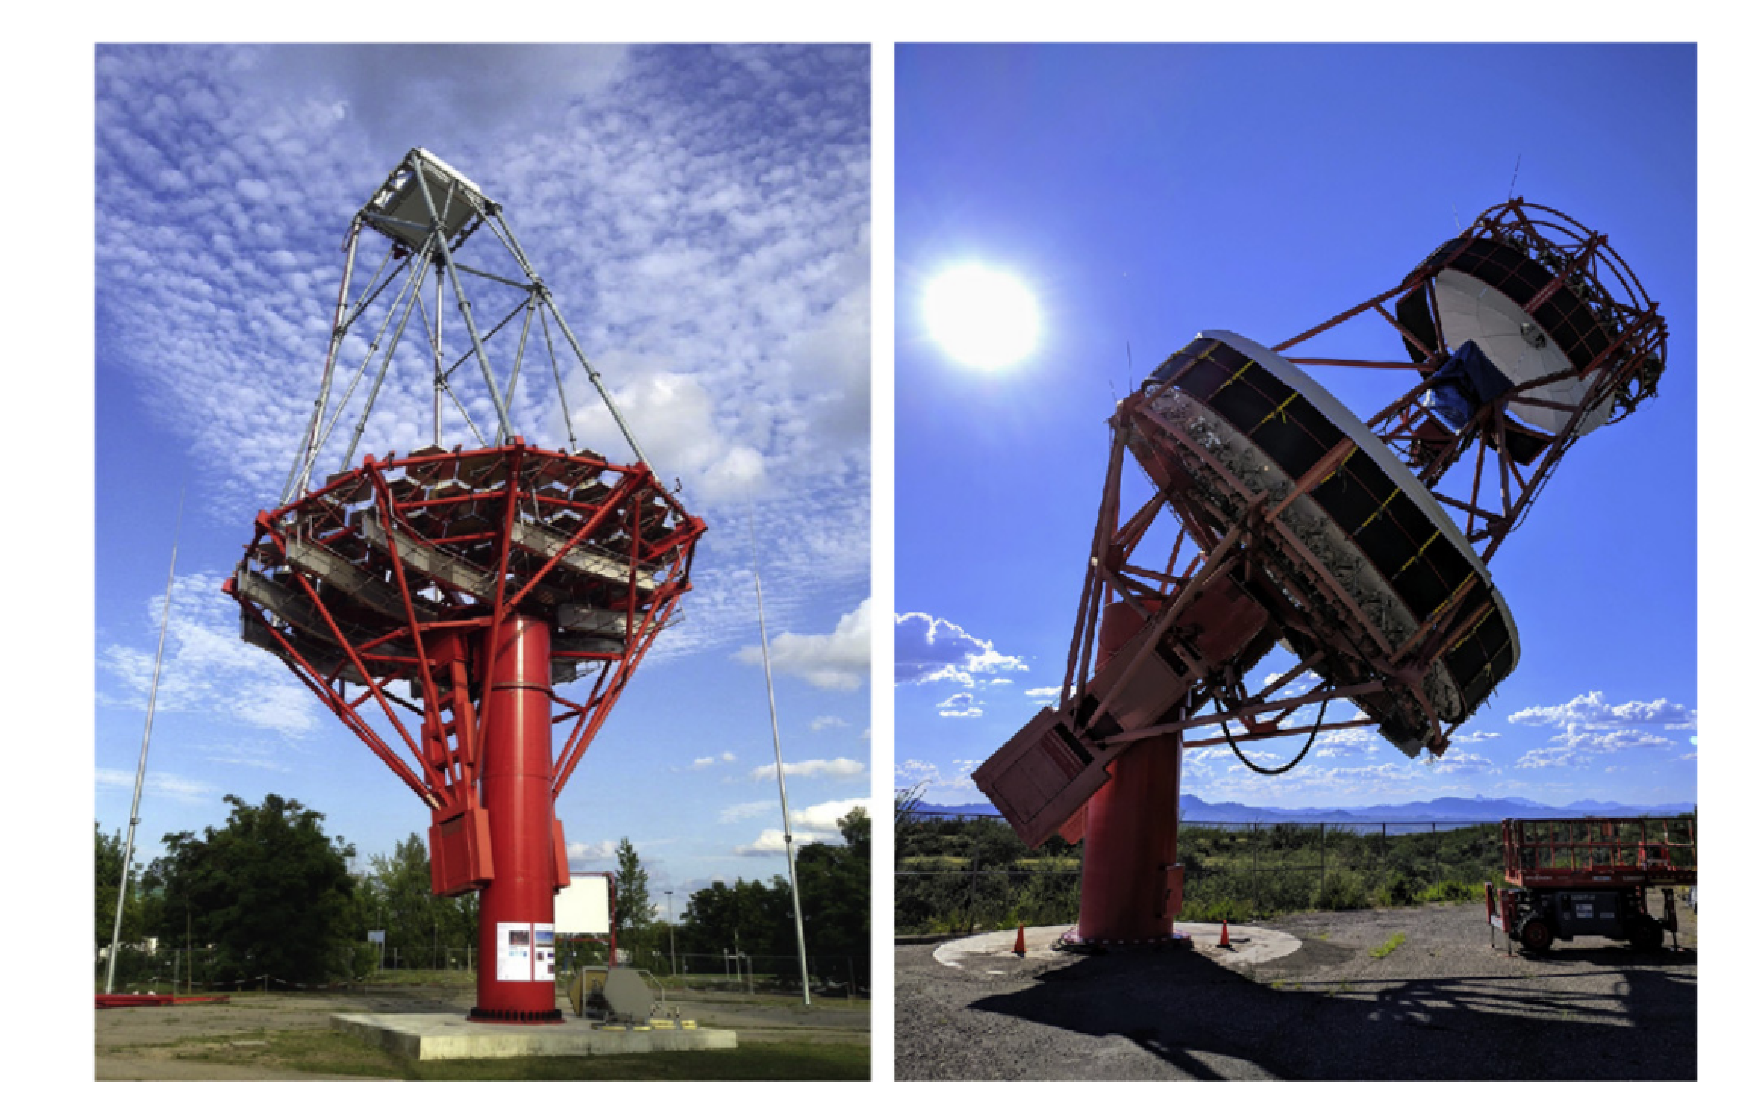
\includegraphics[width=0.7\textwidth]{Pictures/2MSTpictures.pdf}
  \caption{Left: \gls{dcmst} prototype with FlashCam in Adlershof. Right: \gls{scmst} prototype in the Fred Lawrence Whipple Observatory, from \cite{2018MSTandLSTstatus}.}
    \label{fig:2MST}
\end{figure}

\subsubsection{\gls{mst} Optics}

The optical system of the \gls{dcmst} consist on a dish of 86 hexagonal mirror segments of 1.2m length, providing an effective mirror area > 88 m$^2$ and a 12 m diameter reflector. The focal length of the telescope is 16 m.
Different mirror thechnologies are being tested, all based in cold slumping technique, with different layers of materials, coatings and structures. A system of actuators form the \gls{amc} of the \gls{mst} allowing to adjust the mirror position for focusing, however the structure is stiff enough that is not necessary to readjust during observations to maintain the \gls{psf}. The \gls{amc} is used only for the initial mirror adjustment and for maintenance activities or adjust the focal distance for specific observations.

The \gls{scmst} uses a novel aplanatic optical system composed of two aspheric mirrors, which is derived from the exact Schwarzschild solution derived with aplanatic constants $q=2/3$ and $\alpha = 2/3$. The effective focal length of this system is 5.586 m, with a collection area of 50 m$^2$. Both mirrors are segmented as shown in picture \ref{fig:SCMSTmirrors}and the surface is parabolic to minimize astigmatic aberrations at the edge of the \gls{fov}. 


\begin{figure}
\centering
 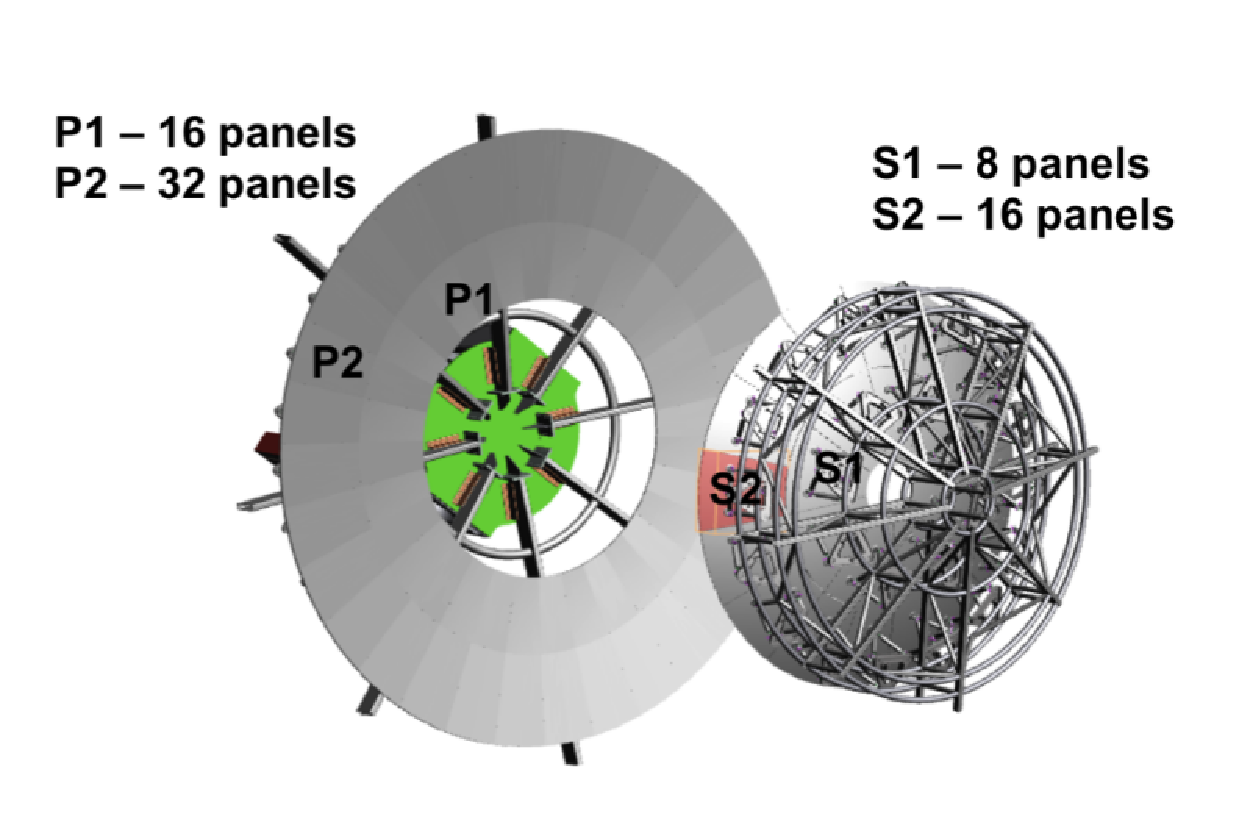
\includegraphics[width=0.7\textwidth]{Pictures/SCMSTMirrors.pdf}
  \caption{Left: \gls{dcmst} Diagram of the optical system of the \gls{scmst}, from \cite{2017SCMSTstatus}.}
    \label{fig:SCMSTmirrors}
\end{figure}

\subsubsection{\gls{mst} Cameras}

For the \gls{scmst} two camera prototypes have been designed and tested in the structure installed in Adlershof and showers have been detected as shown in picture \ref{fig:MSTcamerasimg}.
The first design named FlashCam have 1764 \gls{pmt}-based pixels divided in 147 modules of 12 pixels each. It implements a fully-digital trigger and readout system which allows to define flexible trigger patterns relying on the digitized \gls{pmt} signals. The readout system is designed for a dead-time-free operation with trigger rates up to 30 kHz. FlashCam uses only one gain channel, reducing the required bandwidth for data transfer. 
The second camera design named NectarCAM accounts for 1855 pixels, divided in 256 groups of 7 modules. The camera mechanics and many auxiliary systems have been designed to be equivalent to the \gls{lst} camera. The signal digitizing of NecatrCAM relies on a dedicated Necta ASIC which digitizes the \gls{pmt} signals at sampling speeds of around 1 GHz. It implements a digital trigger based on the binary outputs of individual pixels after comparing their analog signals with a threshold (Level 0 trigger).\\
The camera of the \gls{scmst} is based on \gls{sipm} which allow a very fine pixelization, with 11328 pixels of angular size 0.07º, grouped in 177 modules of $8\times8$ pixels. They are arranged in a slightly parabolic shape and are operated at a temperature that must be controlled to better than 0.1º C. The focal plane of the camera has a diameter of 0.8º m and a \gls{fov} of 8º. The trigger system is based on a two level trigger, where the first level sums the analog signal from 4 adjacent pixels and apply a districminator threshold. The camera is divided in 9 sectors of up to 25 modules and a single backplane board, which receives the trigger signal from 16 modules. A prototype of the \gls{scmst} camera with 24 modules and 2 types of \gls{sipm} has been tested in the \gls{scmst} prototype. The fine pixelization and the module structure of the camera can be appreciated in figure \ref{fig:MSTcamerasimg}. 

\begin{figure}
\centering
 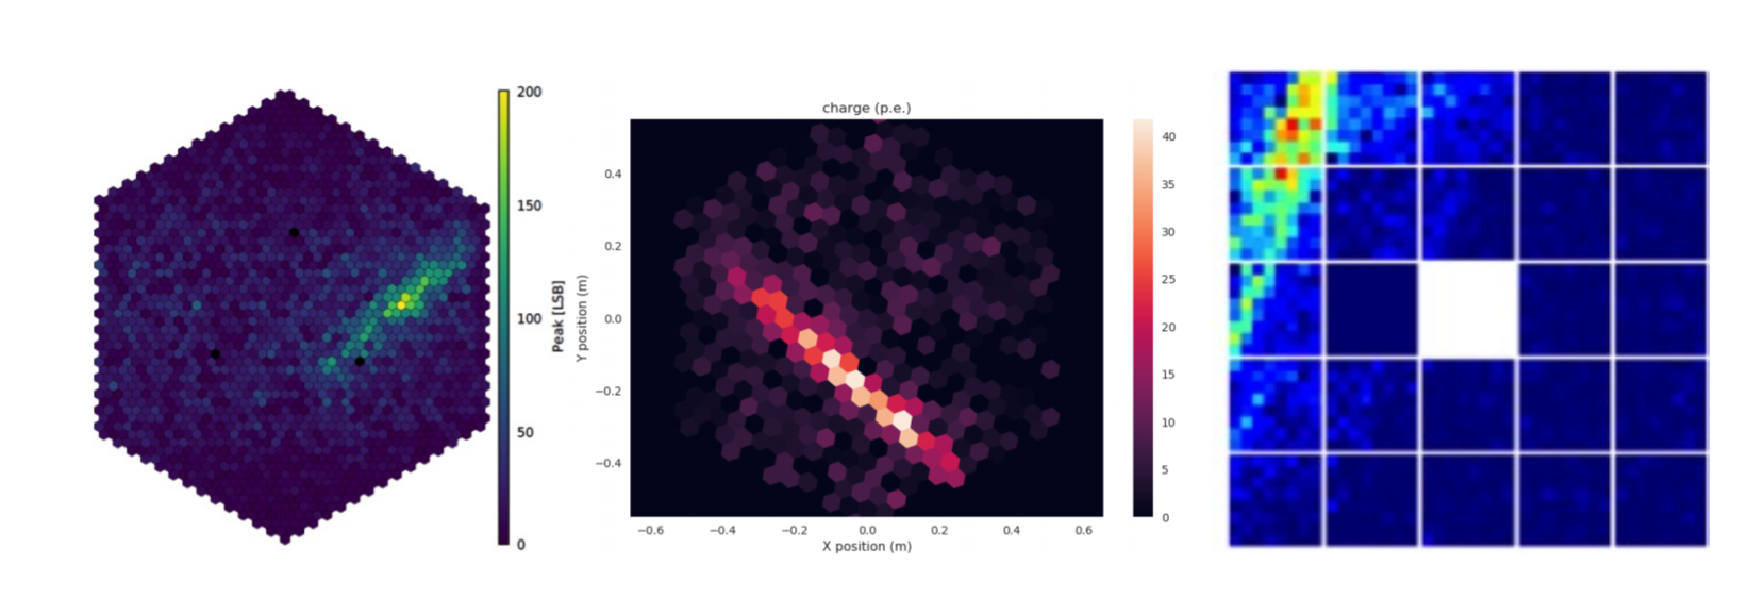
\includegraphics[width=\textwidth]{Pictures/showerimagesMST.pdf}
  \caption{Left: \gls{dcmst} Showers obtained with FlashCam(\textit{left}), NectarCAM(\textit{middle}) and \gls{scmst} camera (\textit{right}) prototypes, from \cite{2019MSTreport}.}
    \label{fig:MSTcamerasimg}
\end{figure}

\subsection{Small Size Telescope (SST)}

The smaller telescopes, \gls{sst} will be the more numerous in the \gls{cta} layout, with more than 70 telescopes in the southern site. These telscopes are dedicated to detect the unfrquent highest energy $\gamma$-rays which in the majority will come from the galactic plane. They need to be spread over a very large area, to catch every possible very energetic $gamma$-ray, but they doesn't need large mirrors because this radiation produces a huge amount of Cherenkov light. The best sensitivity will be achieved at energies greater than 10 TeV. Three \gls{sst} designs have been produced  for \gls{cta}, the ASTRI telescope \cite{2017ASTRItels}, the GCT telescope \cite{2017CHECtels} and the SST-1M telescope \cite{2017SST1M}. In the end, the design of ASTRI telescopes was selected as the one that will be installed in the \gls{cta} layout, but using the GTC CHEC cameras \cite{2017CHECcam}. In this section, summary descriptions of the ASTRI structure and optics design and CHEC cameras are given.

\subsubsection{\gls{sst}-ASTRI Structure}

The optical design of ASTRI telescope is based on a \gls{sc} double mirror configuration, similar to the one described in section \ref{sec:MST} for the \gls{scmst}. A column raises from the base of the telescope and interfaces at the top with the azimuth fork. The fork sustains the elevation assembly, which is composed by the mirror dish, the counterweight and the structure that sustains the two mirrors. The dish is designed to hold the segments of the primary mirrors, which can be individually controlled by actuators. A quadrupod is attached to the dish, which together with a central pole, are joint to the structure that supports the secondary mirror and also serves to counteract deformations due to gravity and wind. The structure for the monolithic secondary mirror accounts for three actuators and three lateral arms which support the transverse components of the mirror's weight. The drive of the azimuth is located at the base of the column. An scheme of the ASTRI structure can be found in picture \ref{fig:SST}. A detailed description of the ASTRI structure design can be fonund in \cite{2013SSTstruct}.

    
\begin{figure}[!htb]
  \minipage{0.4\textwidth}
  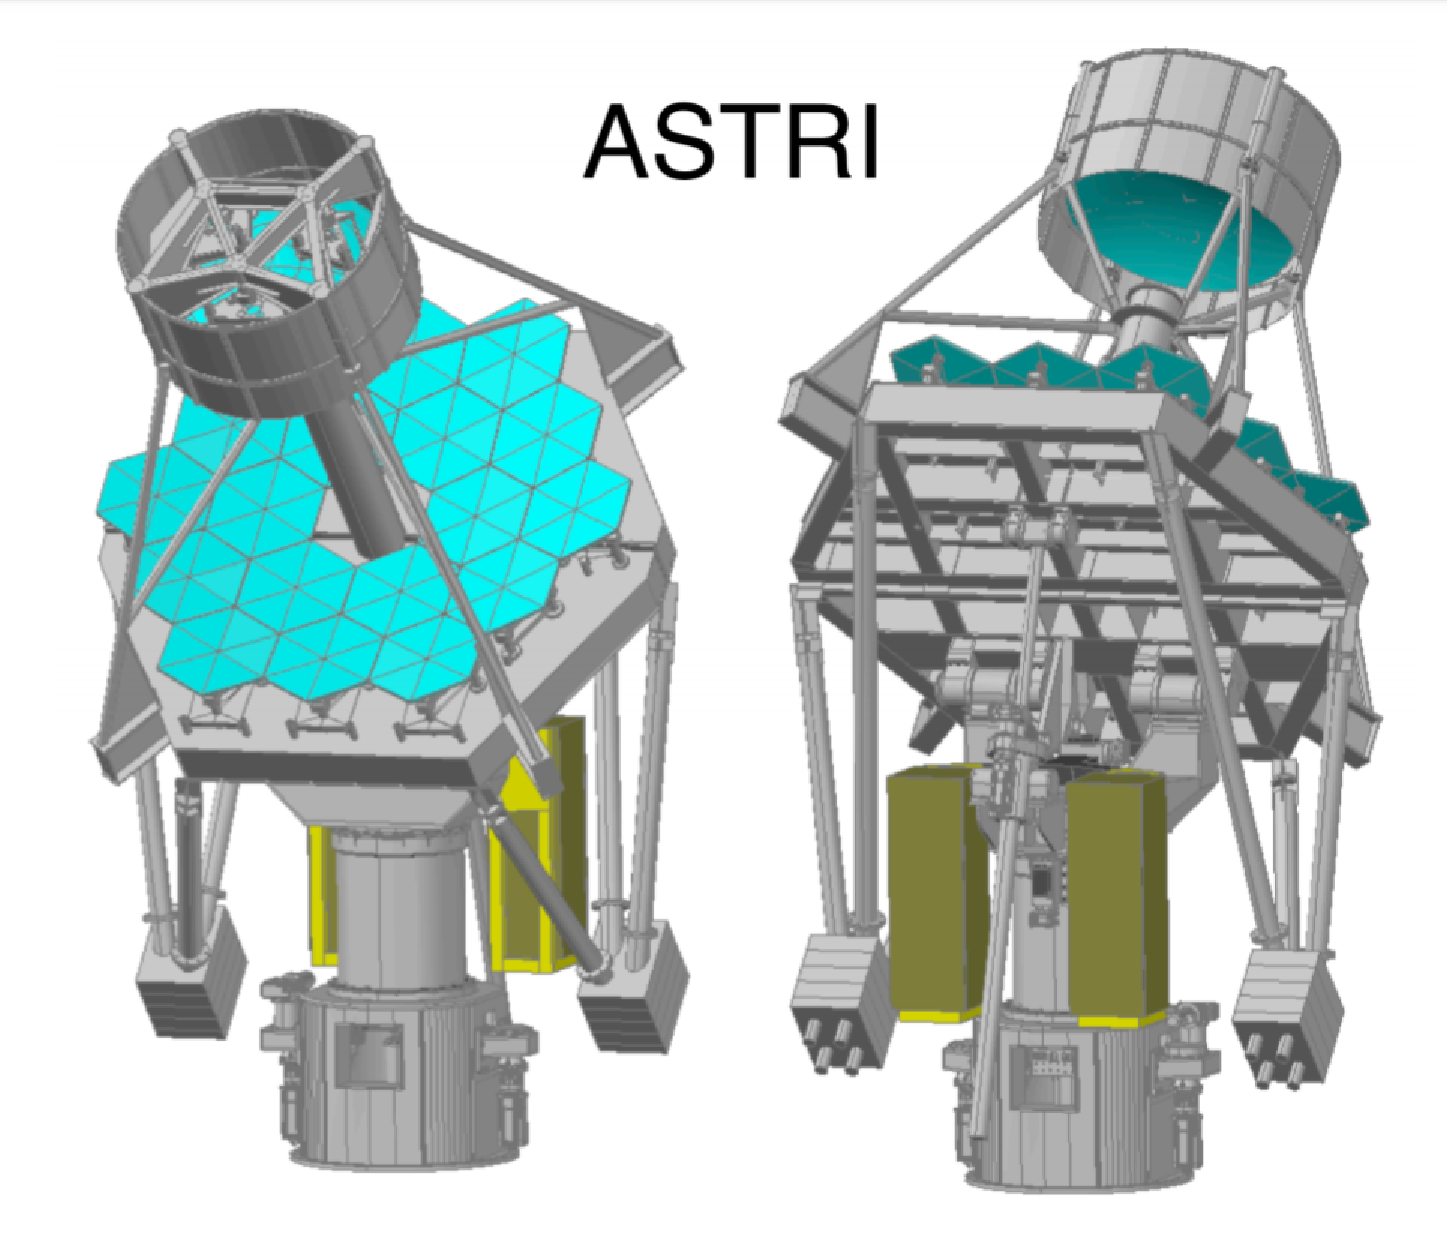
\includegraphics[width=\linewidth]{Pictures/ASTRI.pdf}
  \endminipage\hfill
  \minipage{0.6\textwidth}
  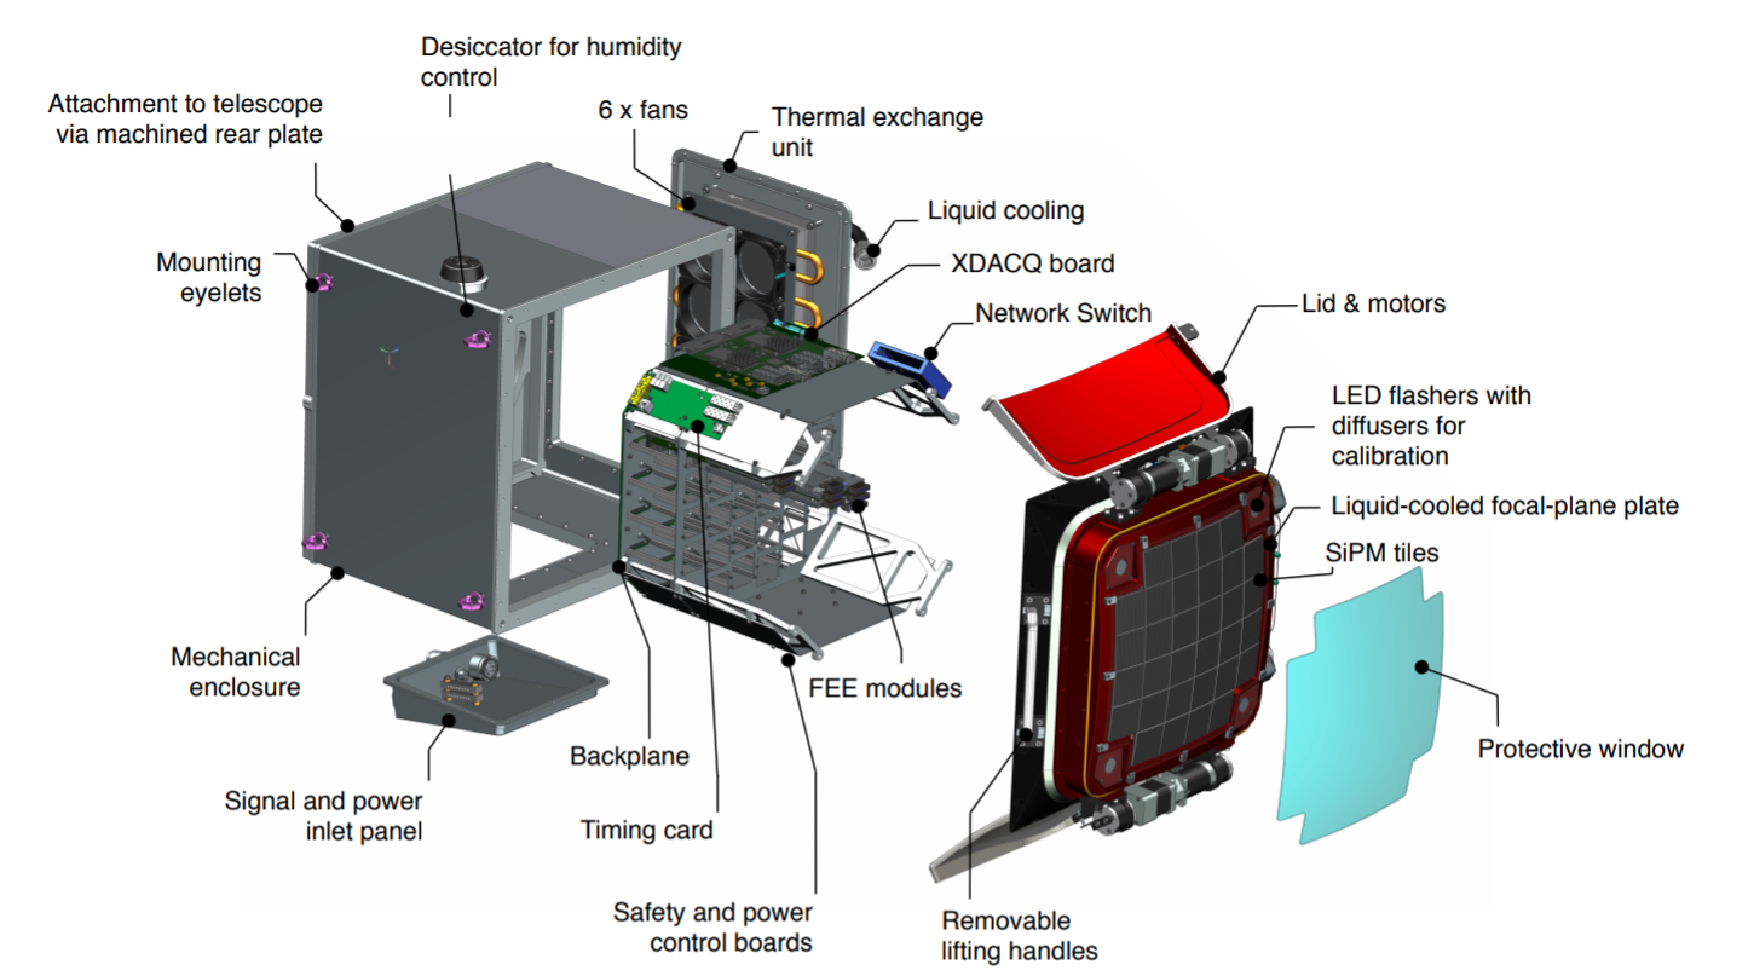
\includegraphics[width=\linewidth]{Pictures/CHECcam.pdf}
  \endminipage\hfill
  \caption{\label{fig:SST} \textit{Left}: General view of the ASTRI telescope structure and electro-mehcanical subsystems, adapted from \cite{2013SSTstruct}. \textit{Right}: CAD model of the \gls{chec} camera from \cite{2017CHECcam} }
\end{figure}

\subsubsection{\gls{sst}-ASTRI Optics}

The \gls{sc} design of the ASTRI telescopes is composed by two mirrors, one primary of 4.3 m diameter composed of an array of hexagonal tiles, and a monolithic secondary mirror of 1.8 m. The primary mirror tiles have been manufactured using a cold slumping replication process. The secondary is make of a hemispherical thick glass shell thermally bent to 2.2 m raiuds of curvature. The focal length of the system if 2.15 m, f/0.5 and the \gls{fov} of the system reaches 10º.\\
The advantages of a double mirror configuration are a better \gls{psf} over a large \gls{fov} and allow better correction of aberrations \cite{2017ASTRItels}.

\subsubsection{\gls{sst}-CHEC Camera}

The \gls{chec} camera was originally designed for the GTC telescope prototype, but finally has been selected to me mounted in the ASTRI sctruture. The camera is composed by 2048 pixels based on \gls{sipm} instrumented in 32 photosensors which comprise 64 pixels of $\sim 6\times6 mm^2$. The digitalization of the waveform is performed by \gls{fee} based on TARGET ASICs \cite{2017TARGETASIC}. It also gives the first trigger level, as the sum of four neighbouring pixels. A backplane provides the power, clock, trigger and data interface of the \gls{fee}. The trigger decision is formed in the backplane by combining trigger signals from all the \gls{fee} modules. In the camera structure, a lid protects the camera from the elments and a cooling system based on the circulation of chilled liquid through the camera focal plane plate and six internal fans. A diagram of the \gls{chec} camera is shown in figure \ref{fig:SST}. A detailed description of \gls{chec} and results from its commissioning can be found in \cite{2017CHECcam}.

\section{Reconstruction and Analysis tools} \label{sec:ctaanalysis}

To obtain the best performance results from \gls{cta} it is very important to have strong software tools, accessible and user friendly, which will allow to analyze the forecoming data. Also, specially in the first parts of the experiment, to calculate the predicted sensitivity shown in section \ref{sec:ctaperformance} it is necessary to produce precise and reliable simulations of the instrument response to the arrival of electromagnetic showers. In this section, the principal softwares for the simulation and analysis of the different levels of \gls{cta} data are described. 

\subsection{Monte Carlo simulations}

\gls{mc} simulations are of great importance for the \gls{iact} technique, where the detection of $\gamma$-rays is indirect and it is necessary to reconstruct the primary parameters from the signal received at the telescopes. Detailed simulations of the development of the \gls{eas} in the atmosphere, combined with simulations of the instrument response to the Cherenkov light produced by those \gls{eas} are used for three main objectives: Separation of $\gamma$ and hadron showers, since hadrons produce the majority of Cherenkov light which reach \gls{iact}, it is necessary to characterize the particular differences between photon and hadron induced showers thanks to the \gls{mc} simulations; and reconstruction of the shower direction and energy of the primary. Comparing the shower parameters to those of the simulated showers applying different methods, like \gls{mva}, \gls{ml} or \gls{dl} among others, the characteristics of the primary particles can be reconstructed.\\
\gls{mc} simulations consists in two phases: The first is the simulation of the \gls{eas} development in the atmosphere, tracking the particles created, the products of their interaction and the amount of Cherenkov light produced. The second part consist on simulating the instruments, taking into account ray tracing, the optical features of the mirrors, the response of the electronics, etc.\\
For \gls{cta}, \gls{mc} simulations have been performed using the programs \gls{corsika}, for the \gls{eas} simulation, and sim\_telarray, for the telescopes response. These two softwares allow to configure a specific array of telescopes with their particular configurations and store only the information of the particles and light from the shower that fall in the surrounding of the telescopes. The current production of \gls{mc} data, with the layout described in section \ref{sec:ctaperformance}, is the named \textit{prod3b-v2} which used \gls{corsika} version 6.9. In the next subsections, a brief description of \gls{corsika} and sim\_telarray is given.

\subsubsection{CORSIKA}

\gls{crosika} is a detailed \gls{mc} program to study the development of \gls{eas} in the atmosphere \cite{1998Corsika}, originally developed for the Kascade experiment \cite{1997Kascade}. The showers can be initiated by different kinds of primary particle, such as photons, protons or other heavier nuclei. The program tries to treat every possible process taking place in the development of \gls{eas} to the present state of our knowledge. It takes into account the transport of particles through the atmosphere and their interactions with air particles. The secondary particles produced are tracked along their trajectories and their parameters are stored when they reach an ob servation level, i.e. the stage of the shower that can be detected by an instrument. They main problem of the simulation of \gls{eas} is the extrapolation of hadronic interactions at the higher energies which cannot be probed in collision experiments. The secondary particles emitted in the extreme forward direction, which are not accessible by colliders, are precisely the more important in \gls{eas} development because they are the one bringin the largest energy fraction to the atmosphere. The extrapolations must therefore rely on different theoretical models. To study the systematics of such models, in \gls{corsika} there are five different hadronic interaction models available. For \gls{cta} prod3b-v2 the model used was QGSJET-II \cite{2006QGSJET}. An example of three different showers simulated with \gls{corsika} is shown in picture \ref{fig:corsika}.

\begin{figure}[!htb]
  \minipage{0.33\textwidth}
  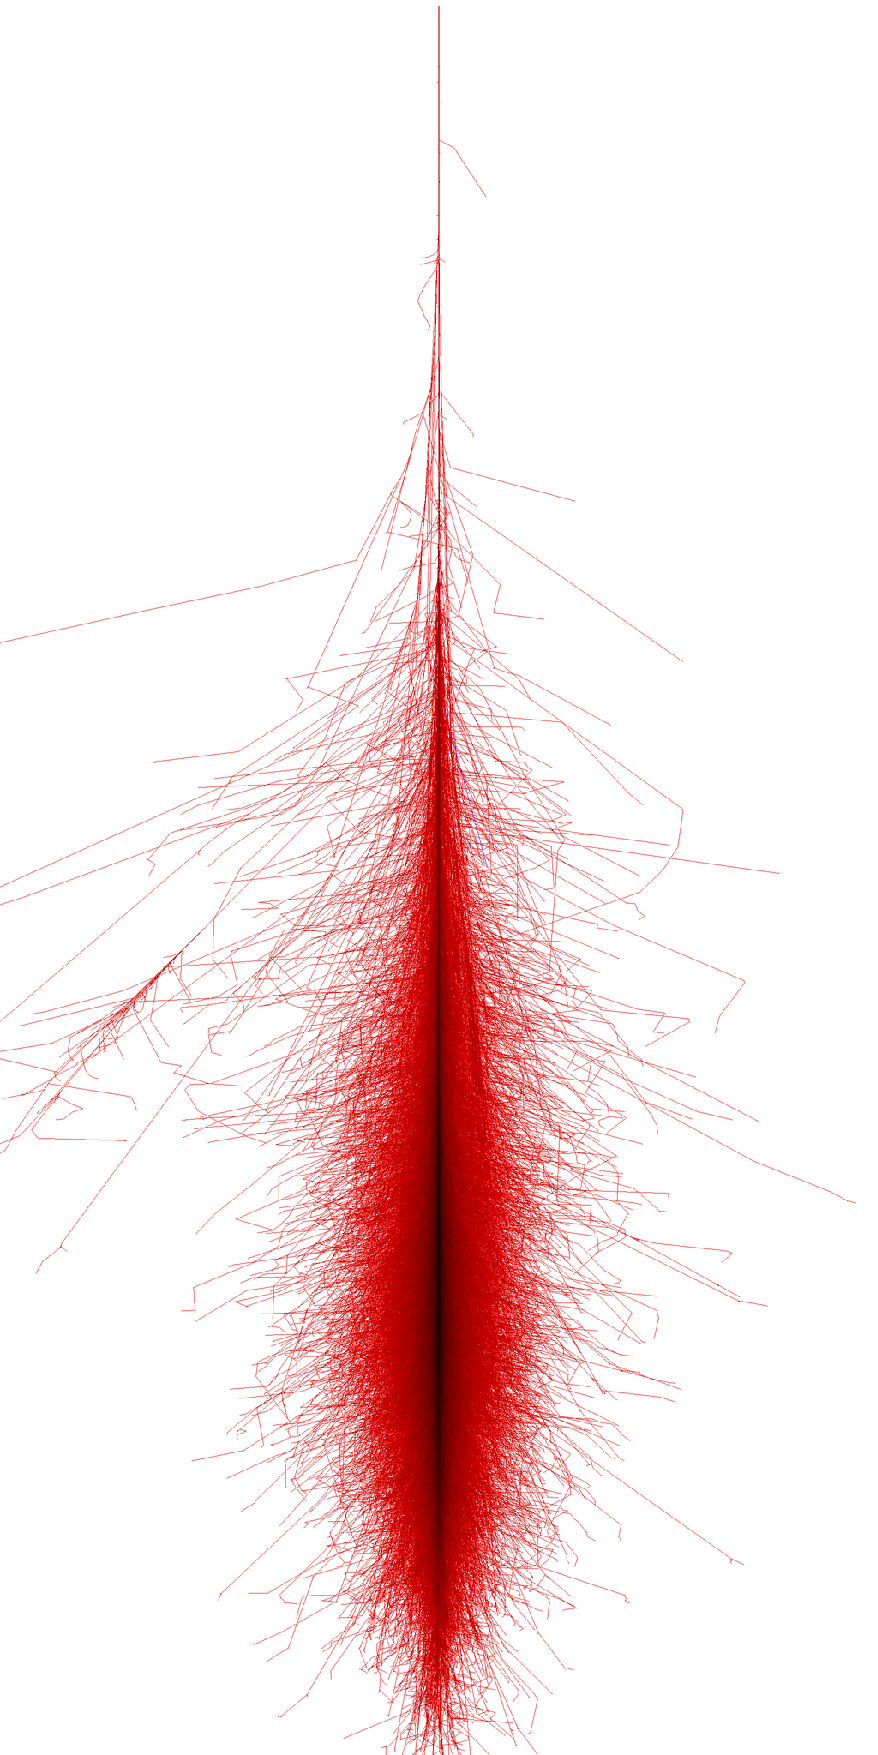
\includegraphics[width=\linewidth]{Pictures/photon_12_0deg.pdf}
  \endminipage\hfill
  \minipage{0.33\textwidth}
  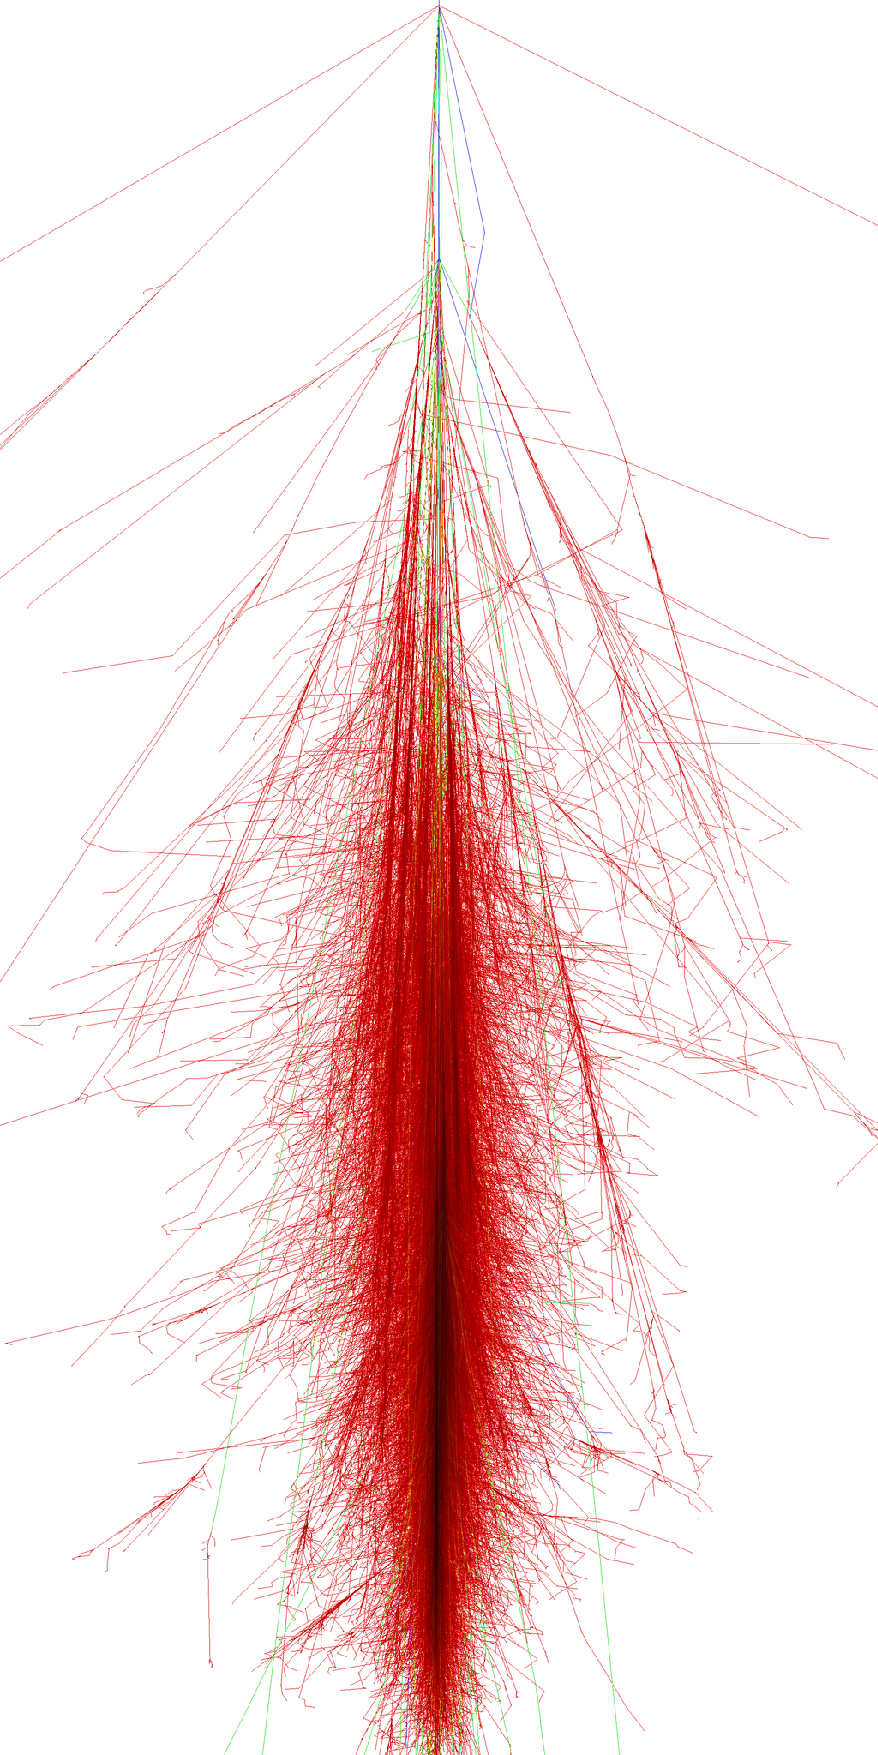
\includegraphics[width=\linewidth]{Pictures/proton_12_0deg.pdf}
  \endminipage\hfill
    \minipage{0.33\textwidth}
  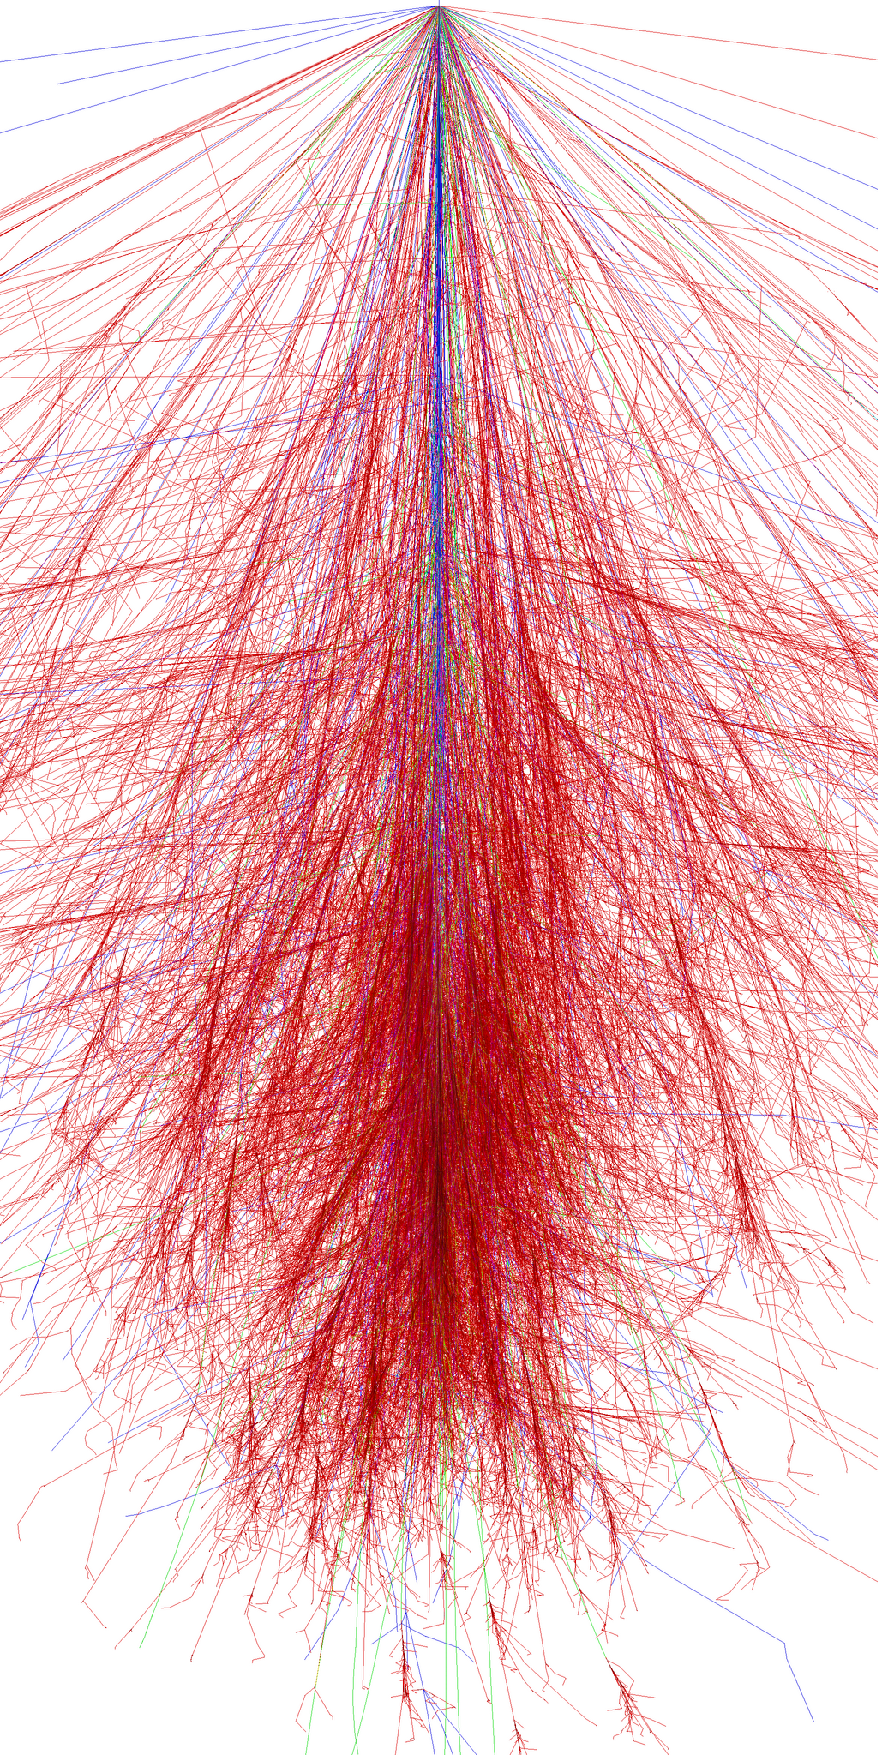
\includegraphics[width=\linewidth]{Pictures/iron_12_0deg.pdf}
  \endminipage\hfill
  \caption{\label{fig:corsika} Photon (left), proton (center) and iron (right) produced showers for a primary energy of 1 TeV and 0º zenith angle, simulated with \gls{corsika} from \cite{corsikaimages}.}
\end{figure}

\subsubsection{sim\_telarray}
\subsection{Low level analysis: ctapipe}
\subsection{Science analysis: ctools}

\end{document}
